\documentclass[11pt, titlepage]{article}
\usepackage{geometry}        
\geometry{letterpaper}    
\usepackage[parfill]{parskip}  
\usepackage{graphicx}
\usepackage{amssymb}
\usepackage{epstopdf}
\usepackage{amsmath}
\DeclareGraphicsRule{.tif}{png}{.png}{`convert #1 `dirname #1`/`basename #1 .tif`.png}
\usepackage{float}
 \usepackage[usenames,dvipsnames]{pstricks}
\usepackage{epsfig}
 \usepackage{pst-grad} % For gradients
 \usepackage{pst-plot} % For axes
 \usepackage[space]{grffile} % For spaces in paths
 \usepackage{etoolbox} % For spaces in paths
\makeatletter % For spaces in paths
\graphicspath{ {images/} }
\usepackage{titling}
\usepackage{fontspec}
\usepackage{pgfplots}
\usepackage{eso-pic}
\usepackage{soul}
\newcommand\AtPageUpperRight[1]{\AtPageUpperLeft{%
   \makebox[\paperwidth][r]{#1}}}
\usepackage{caption}
\usepackage[version=4]{mhchem}

\newfontfamily\headingfont[]{Calibri}
\renewcommand{\maketitlehooka}{\headingfont}

 \patchcmd\Gread@eps{\@inputcheck#1 }{\@inputcheck"#1"\relax}{}{}
\makeatother
\usepackage{pst-node,pst-circ}

\usepackage[most]{tcolorbox}
\usepackage{comment}
\usepackage[colorlinks=true, pdfstartview=FitV, linkcolor=blue, 
            citecolor=blue, urlcolor=blue]{hyperref}
            
\usepackage{afterpage}
\usepackage[pagecolor=none]{pagecolor}

%\includeonly{Chapter1}
\usepackage{fancyhdr}
\pagestyle{fancy}
\rfoot{www.crashentry.com}

\makeatletter
\newcommand\HUGE{\@setfontsize\Huge{38}{47}} 
\makeatother



% ------------------- Title and Author -----------------------------
\title{
\HUGE\textbf{\textcolor{white}{{\addfontfeature{LetterSpace=5.0}CRASH ENTRY}}} \\
\Huge\textbf{\textcolor{white}{{\addfontfeature{LetterSpace=7.0}PHYSICS}}
}}
\author{}
\date{}
\begin{document}

\definecolor{entryscheme}{HTML}{FF0012}
\newpagecolor{entryscheme}\afterpage{\restorepagecolor}



\begin{comment}
\AddToShipoutPictureBG*{%
  \AtPageUpperRight{\raisebox{-\height}{\frame{
\includegraphics[width=8cm]{crashentry}}}}}

\makeatletter
\renewenvironment{quotation}
           {\list{}{\listparindent 1.5em%
                    %\itemindent    \listparindent
                    %\rightmargin \leftmargin
                    \parsep        \z@ \@plus\p@}%
            \item\relax}
           {\endlist}
\makeatother
\end{comment}



\maketitle




%\section*{Introduction}
This is intended to give you a very brief introduction to a lot of the concepts in Physics you will need to approach the BMAT.  However, since the number of edge cases is so vast this is no substitute for actual understanding, and there will undoubtedly be concepts missed here that could come up in the BMAT.  The best thing you can do is to just practice these concepts with real questions.  These include past GCSE, A-level and BMAT papers.  We have attempted to include the essentials of the course specification, so use that along with this booklet to supplement your learning.

\section{Electricity}
With electricity, we need to make it clear what it is and what causes it.  In every electronic device, incredibly intricate circuits are created which carry an electric current, which is the movement of negatively charged electrons.  This movement carries with it energy, which powers the device.

Current, $I$ in a circuit is how fast charge travels around the circuit in a given time, but we can also relate this to two other quantities, resistance, $R$,  and voltage, $V$.  Voltage is the energy carried per unit charge, and resistance can be defined as anything slowing the flow of charge.

In effect
\begin{description}
\item[Voltage] How much energy is being carried.
\item[Current] How fast it's carried around the circuit.
\item[Resistance] How difficult is it to carry around the circuit.
\end{description}  

We can relate all three through Ohm's Law
\begin{equation*}
\mathbf{V=IR}.
\end{equation*}

\subsection{Circuits}
Measuring these values from a circuit diagram commonly appears in the BMAT.  In a circuit diagram there are a few symbols you need to know.  

\subsubsection*{Lamp}

\begin{figure}[H]
\centering
\begin{pspicture}(-2,-1)(2, 1)
%Lamps
\pnode(-2, 0){Lamp1}
\pnode(2, 0){Lamp2}
\lamp(Lamp1)(Lamp2){}
\end{pspicture}
\end{figure}

These emit light and are a key feature of most circuits that have appeared in the past papers.  Each bulb has a resistance and typically the brightness is proportional to the power passing through it.

\subsubsection*{Resistor}
\begin{figure}[H]
\centering
\begin{pspicture}(-2,-1)(2, 1)
%Lamps
\pnode(-2, 0){Lamp1}
\pnode(2, 0){Lamp2}
\resistor(Lamp1)(Lamp2){}
\end{pspicture}
\end{figure}

One of the major sources of resistance in a circuit.

\subsubsection*{Diode}
\begin{figure}[H]
\centering
\begin{pspicture}(-2,-1)(2, 1)
%Lamps
\pnode(-2, 0){Lamp1}
\pnode(2, 0){Lamp2}
\diode(Lamp1)(Lamp2){}
\end{pspicture}
\end{figure}

This is likely to be one you haven't encountered before, but its remarkably simply.  If current is flowing in the direction the diode arrow points then nothing changes.  If however it is moving in the opposite direction then no current can flow through the diode effectively breaking the circuit.

\subsection*{Switch}
\begin{figure}[H]
\centering
\begin{pspicture}(-2,-1)(2, 1)
%Lamps
\pnode(-2, 0){Lamp1}
\pnode(2, 0){Lamp2}
\switch[dipolestyle=normal](Lamp1)(Lamp2){}
\end{pspicture}
\end{figure}

A switch just allows current to either flow through a path in the circuit or not.  If it's open, as it is here, then no current can flow.  If it's closed then current will flow.


\subsubsection*{Ammeter}
\begin{figure}[H]
\centering
\begin{pspicture}(-2,-1)(2, 1)
%Lamps
\pnode(-2, 0){Lamp1}
\pnode(2, 0){Lamp2}
 \circledipole[labeloffset = 0](Lamp1)(Lamp2){A}
\end{pspicture}
\end{figure}

These measure the current flowing through a circuit and therefore will always lie in series with the actual circuit.

\subsubsection*{Voltmeter}
\begin{figure}[H]
\centering
\begin{pspicture}(-3,-3)(3, 1)
%Lamps
\pnode(-2, -2){Lamp1}
\pnode(2, -2){Lamp2}
 \circledipole[labeloffset = 0](Lamp1)(Lamp2){V}
 %Wires
 \pnode(-2, 0){Wire1}
 \pnode(2, 0){Wire2}
 \wire(Wire1)(Lamp1)
 \wire(Wire2)(Lamp2)
 \pnode(-3, 0){LampX}
 \pnode(3, 0){LampY}
 \lamp(LampX)(LampY){}
\end{pspicture}
\end{figure}

A voltmeter measures the potential resistance, or voltage drop, between two points in a circuit.  Here it is measuring the potential distance across the lamp pictured.  If this lamp were removed we would measure an incredibly low potential difference as, using $V=IR$, a wire has a very low resistance so the voltage will also be very low.

\subsection{Series and Parallel Circuit}
There are two types of circuit configuration you need to be aware of.  Firstly, series circuit of which an example is shown below.

\begin{figure}[H]
\centering
\begin{pspicture}(-3,-3)(3, 2)
%Lamps
\pnode(-3, 2){batteryX}
\pnode(3, 2){batteryY}
\battery(batteryX)(batteryY){}
\pnode(-3, -2){lampX}
\pnode(3, -2){lampY}
\lamp(lampX)(lampY){}
\wire(batteryX)(lampX){}
\wire(batteryY)(lampY){}
\end{pspicture}
\end{figure}

In these the current flows clockwise, from the positive to negative terminal.  A quick rule to remember is if we're adding resistors in a series circuit, we just sum up the resistances to get the total resistance
\begin{equation*}
\mathbf{R=R_1 + R_2 + R_3 + ...}
\end{equation*}

An example of a parallel circuit would be
\begin{figure}[H]
\centering
\begin{pspicture}(-3,-3)(3, 3)
%Lamps
\pnode(-3, 2){batteryX}
\pnode(3, 2){batteryY}
\battery(batteryX)(batteryY){6V}
\pnode(-3, -2){lampX}
\pnode(3, -2){lampY}
\resistor(lampX)(lampY){$2\Omega$}
\wire(batteryX)(lampX){}
\wire(batteryY)(lampY){}

\pnode(-3, 0){Lamp1X}
\pnode(3, 0){Lamp1Y}
\resistor(Lamp1X)(Lamp1Y){$3\Omega$}
\end{pspicture}
\end{figure}

In this case the current splits at the first path, depending on the resistance of each.  We can calculate this using $V=IR$, so the upper path will have a current of 2 A, while the lower one will have a current of 3 A. 

If we wanted to calculate the total resistance of this circuit we can't just add up the resistances however.  We use
\begin{equation*}
\mathbf{\frac{1}{R} = \frac{1}{R_1} + \frac{1}{R_2} + \frac{1}{R_3} + ... }.
\end{equation*}
So for our parallel circuit we have $\frac{1}{3} + \frac{1}{2} = \frac{5}{6}$, so a total resistance of $\frac{6}{5}$.  Using Ohm's law this means the initial current is $6 \div \frac{6}{5}$ or 5 A.  This is just the sum of the split currents. 

Voltage however does not split and will be equal in each branch.  This has an important consequence that in the above circuit each lamp will be equally bright, even if we add another lamp with another parallel branch.  However if we add more lamps to the series circuit, they will all drop in brightness.

Parallel circuits are quite tricky but remember these rules:
\begin{itemize}
\item Current splits according to the resistance of each branch.
\item Voltage does not split at the branches.
\end{itemize}

So these two are fairly straightforward but you'll undoubtedly be asked much more complex questions in the actual exam.

\subsection*{Example}
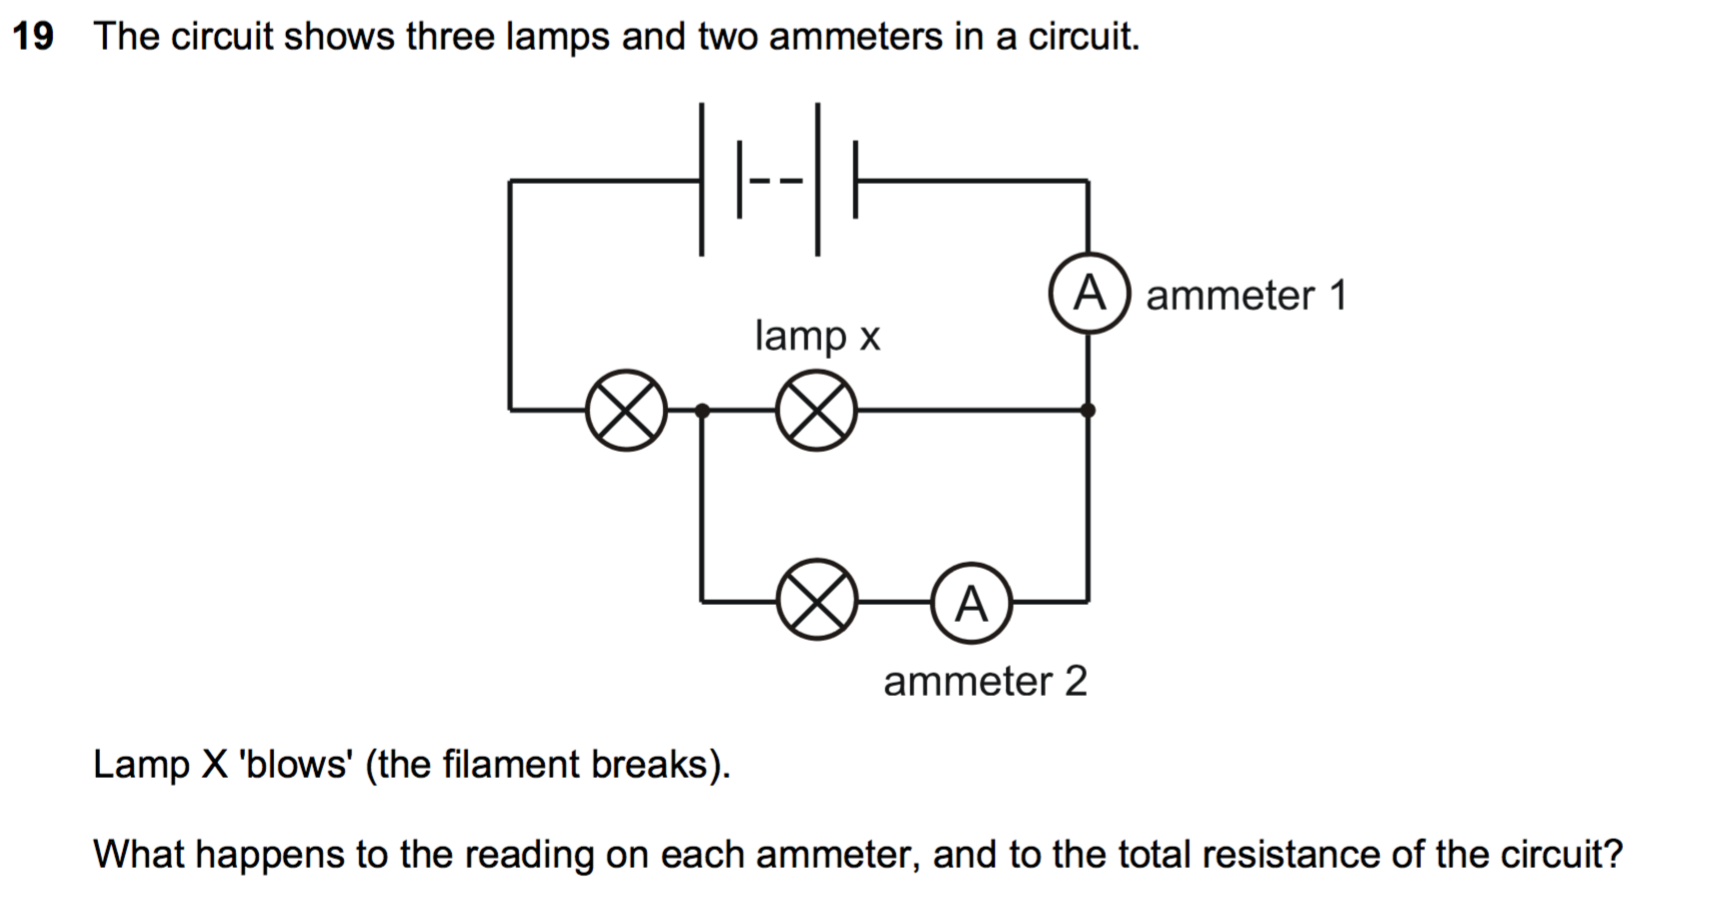
\includegraphics[width=\textwidth]{2012q19}

Here's a quick example to illustrate these points.  If Lamp X blows then current can no longer move along that path, so if you think about it we effectively have a series circuit now.  All the current now flows into Ammeter 2, rather than being split, so it's reading will increase, but how do we compare the resistance.  

First we need to calculate the resistance before the lamp blew.  Assume the lamps all have resistance X, so firstly calculate the resistance of the parallel component.

\begin{equation*}
\frac{1}{X} + \frac{1}{X} = \frac{2}{X}
\end{equation*}

So we have a resistance of $\frac{X}{2}$, which we add to the resistance off the other lamp yielding $X + \frac{X}{2} = \frac{3X}{2}$.  After the bulb breaks, we have a resistance of $2X$, as we can just add the resistances since it's now effectively a series circuit.  So the total resistance increases and using Ohm's Law, the current will decrease so ammeter 1's value decreases.  

\subsection{Short Circuit}
You've undoubtedly heard of short circuit, when something you own just no longer works correctly, and this is a concept that has been tested a number of times in the exam. 

\begin{figure}[H]
\centering
\begin{pspicture}(-3,-3)(3, 3)
%Lamps
\pnode(-3, 2){batteryX}
\pnode(3, 2){batteryY}
\battery(batteryX)(batteryY){}
\pnode(-3, -2){lampX}
\pnode(3, -2){lampY}
\lamp(lampX)(lampY){}
\wire(batteryX)(lampX){}
\wire(batteryY)(lampY){}

\pnode(-3, 0){Lamp1X}
\pnode(3, 0){Lamp1Y}
\switch(Lamp1X)(Lamp1Y){}
\end{pspicture}
\end{figure}

 If we were to close the switch, remembering that a wire has an incredibly low resistance (effectively nothing), then all the current will flow through that path, entirely bypassing the lamp.  Current will favour the path of least resistance and if this happens then the lamp won't work.

\subsection{Power and Energy}
We've mentioned voltage as being a measure of how much energy is being carried, and current as the speed of that transfer, so to calculate how much power is being generated in the circuit we can use
\begin{equation*}
\mathbf{P=VI}.
\end{equation*}
Typically you'll have to use this with Ohm's Law, $V=IR$, depending on which values you've been given.

To calculate the total energy transferred you simply multiply the power by the time taken,
\begin{equation*}
E = Pt.
\end{equation*} 

\subsection{Transformers}
Electromagnetic induction is how electricity can be generated in a conductor.  By applying a changing magnetic field to a coil of wire, for example, a voltage will be induced within the wire.  Normally this will be achieved by rotating a coil of wire in a magnetic field, inducing a voltage across the coil.  Understanding this is key to understanding how transformers work.

Not all devices will work at all voltages, and in some cases this can be incredibly harmful to the devices.  If, for example with a bulb, the voltage is too high this could cause the bulb to blow.  We use transformers to reduce the voltage down to safe levels.

A transformer is made up of two coiled wires.  By varying the current in the primary coils, this induces a changing magnetic field which induces a current in the secondary coils.  The voltage induced across the second depends on the \textbf{number of coils in each}.  They are related through
\begin{equation*}
\mathbf{\frac{V_p}{V_s} = \frac{n_p}{n_s}},
\end{equation*}
where $n_p$ and $n_s$ are the number of coils on the primary and secondary wires respectively.  

We often assume 100\% efficiency with transformers implying all power is transferred, or
\begin{equation*}
\mathbf{V_pI_p = V_sI_s.}
\end{equation*}



\section{Motion and Energy}
One of the key skills in physics is the ability to describe the motion of objects according to Newton's laws of motion.  This isn't intended to be a full comprehensive overview of all of Newtonian physics however, merely a refresher to guide you on the types of questions typically tackled in the BMAT.  If you're struggling on a certain topic, free online resources will be linked to give a more thorough introduction.  Most of what we're going to cover in this section should be familiar to you from GCSE, but there are some slight details that you might be unaware of if you haven't done the AS level.

\subsection{Kinematics}
Starting out with the very basics, for an object with no force applied, moving with a constant speed, $v$ we can describe this in terms of the distance it travels, $d$ and the time taken, $t$.  This is 
\begin{equation*}
\mathbf{v = \frac{d}{t}}.
\end{equation*}
This is an absolutely fundamental equation to remember for all sections.

If we're changing our speed mid journey however, this equation will not hold so we need to use the equation for acceleration, which is
\begin{equation*}
\mathbf{a = \frac{\rm{\mathbf{change\; in\; velocity}}}{\rm{\mathbf{time}}} = \frac{v_1 - v_0}{t}}.
\end{equation*}

Here, $v_1$ would be the speed you start at and $v_0$ is the speed you end up at.  So we now have a way of measuring just how fast you are changing your speed.

Each of these will have an associated direction, which are known as vectors.  To visualise this just imagine two cars driving in opposite directions, with equal speeds.  If you draw an arrow showing their movement, they will be in opposite directions of equal sizes.  If one car is larger than the other it will have a larger arrow.  A vector can be visualised as this arrow.

When dealing with vectors we refer to the speed as the velocity, speed with a direction.  

\subsection{Distance-Time and Velocity-Time Graphs}
One type of question that has popped up in the past are those which require you to analyse velocity-time and distance-time graphs.  You need to be able to calculate gradients and the area under graphs.  

How these different graphs relate to each other is a bit tricky to explain without calculus but the gradient of a graph is the rate of change of that quantity.

We know velocity is the rate of change of distance with time, so the gradient of a distance-time graph will be the velocity.  Acceleration is the rate of change of velocity with time, so the gradient of a velocity-time graph will be the acceleration.  

To go back, we take the area under the curve, so the area under a velocity-time graph will be the total distance travelled and the area under an acceleration-time graph will be the total velocity change.

\subsection*{Example 1}

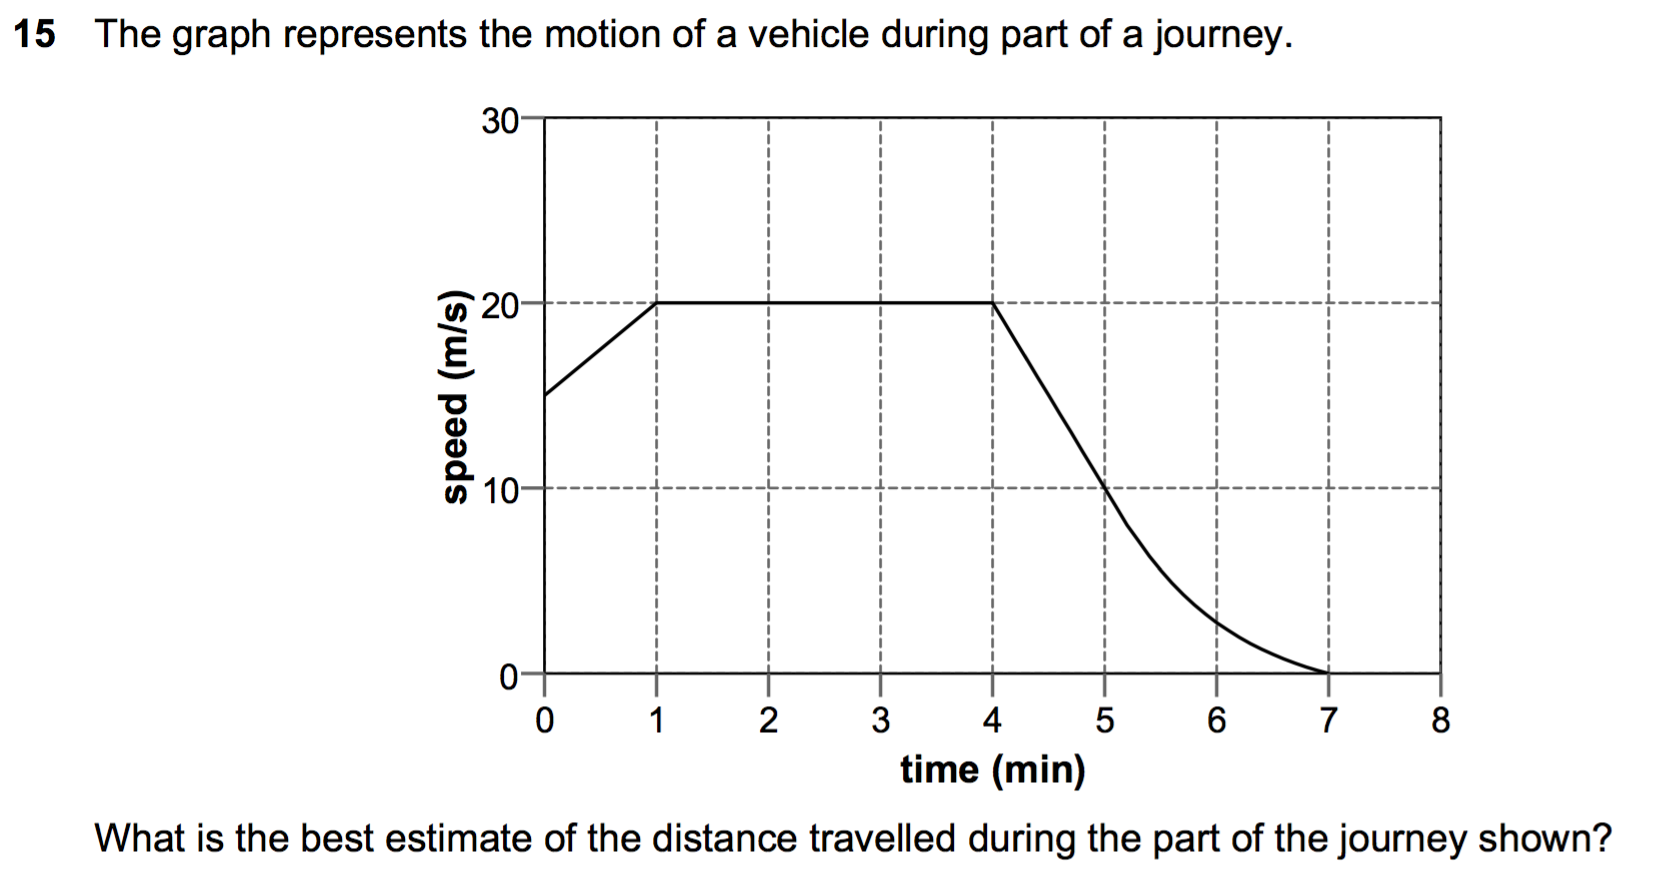
\includegraphics[width=\textwidth]{vt}

Calculating the area under a graph is a little involved, but the easy way is just to add the area of each of the dotted boxes shown on this graph to get the distance.  Due to the curved area you will have to use some assumptions, or model it as a straight line and correct later.

\subsection*{Example 2}

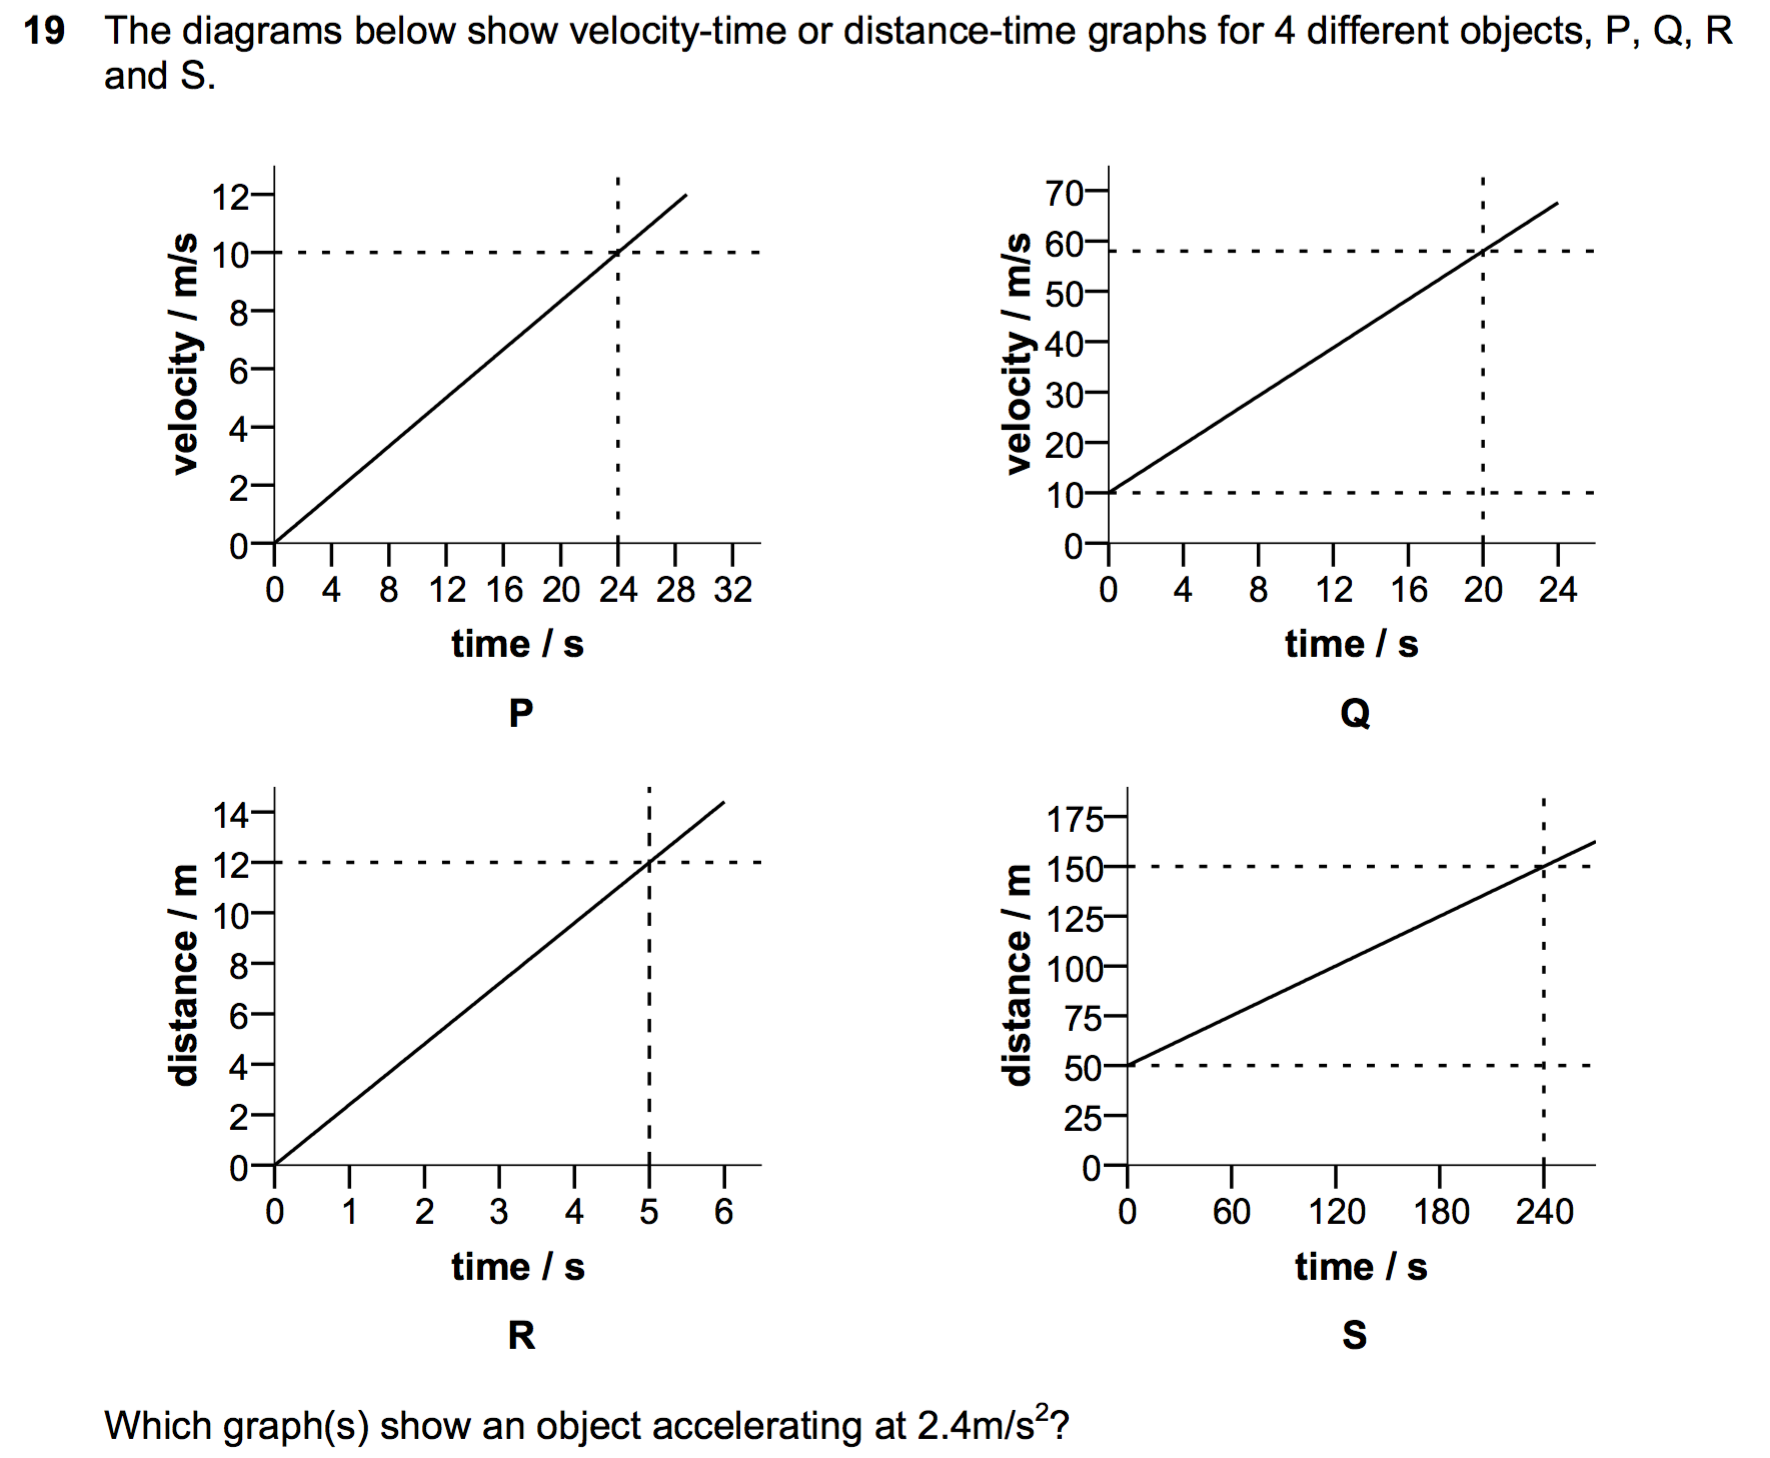
\includegraphics[width=\textwidth]{vt+dt}

This shows four graphs and we want to find an accelerating object.  The bottom two are distance-time graphs so will have no change in velocity as they are straight lines, therefore no acceleration.  The top two however are accelerating as they have an increase in velocity.  To calculate the gradient just take the total velocity change and divide it by the time, which is easy due to the guides to the axis.

\subsection{SUVAT}
As an aside it's probably best to go over the SUVAT equations.  The official BMAT website states that while these aren't required, they're useful.  However there have been questions that have required their use in the past, so its better to be safe than sorry and to learn these.  SUVAT equations are 5 equations describing the relationship between 5 different variables.  These are:
\begin{itemize}
\item Initial Velocity, $u$
\item Final Velocity, $v$
\item Acceleration, $a$
\item Distance Travelled, $s$
\item Time Taken, $t$
\end{itemize}

These equations are
\begin{equation*}
\begin{aligned}
v&=u+at\\
v^2&=u^2+2as\\
s&=ut+\frac{1}{2}at^2\\
s&= \frac{1}{2} (v+u)t\\
s&= vt - \frac{1}{2}at^2\\
\end{aligned}
\end{equation*}



%\begin{tcolorbox}[breakable,colback=white,colframe=red,width=\dimexpr\textwidth+12mm\relax,enlarge left by=-6mm]

%\end{tcolorbox}


\subsection{Forces}
You'll have to become well acquainted with Newton's three laws of motion to solve a lot of problems on the BMAT. 

\begin{enumerate}
\item{Without the application of an external force, a body will continue to move at a constant velocity in an inertial reference frame.}
\item{$\mathbf{F=ma}$}
\item{When a body exerts a force on a second body, the seconds body exerts an equal and opposite force on the first body.}
\end{enumerate}

Lets break them down quickly.  The first is simply stating that any object will continue to move at a constant velocity, unless you act on it with a force.  If for example, we were flying through space with no gravity, we'd continue travelling at the same speed forever.  This is called \textbf{inertia}.

The second is the relationship between acceleration and the force applied, as a force will change your velocity.  Remember this equation!

For the third, if you press your hand against the table, the table is exerting a force on your hand equal to the one you're applying.  Otherwise your hand would just pass straight through the table.

If you have two opposite forces applied to an object, we just subtract one from the other to get the \textbf{resultant force}.  Gravity exerts a force on you all the time but since we are standing on the ground, which via Newton's 3rd law exerts an equal and opposite force, we have 0 resultant force acting on us.

\subsection{Momentum}
Another key concept to remember is that of momentum.  Momentum, $P$ is a quantity that relates to your mass and your velocity by
\begin{equation*}
\mathbf{P=mv}.
\end{equation*}
Every object carries momentum depending on how fast it's travelling and its mass, and this is always conserved no matter what!  If two objects collide and move off at different velocities, they will each have different momenta, but the sum of their momenta before they collided, will be equal to the sum after they collided.  We can describe the force exerted on each object during the collision as the \textbf{rate of change of their momenta}, i.e
\begin{equation*}
\mathbf{F=\frac{\Delta P}{\Delta t}},
\end{equation*} 
where $t$ is time and the delta represents the change in that value.



\subsection{Gravity}

To force gravity exerts is your \textbf{weight}.  This is different from your \textbf{mass} as your mass is the amount of matter in your body while your weight is dependent on the gravity of the planet.  We can calculate weight using
\begin{equation*}
\mathbf{W=mg},
\end{equation*}
where $m$ is your mass and $g$ is the gravitational field strength of the planet (which in the absence of any other force will be the speed you accelerate at).  In the BMAT this is approximated to 10 N/kg (this will be given to you).

Now we need to tackle how someone falling through the air would act.  When falling initially you'll be accelerating due to the force of gravity, but as you fall, the air will apply an opposite force to counteract this.  Initially this force will be much greater than gravity, causing you to decelerate, but as you slow down the air resistance also reduces, until it's equal to the force of gravity.  You will then have a resultant force of 0 N and you will be falling at your \textbf{terminal velocity} (Remember Newton's first law!  You don't need a force to have a velocity).

\subsection{Energy}
We can't create or destroy energy, we can only transform it into another form, it is always conserved.  It comes in many different forms such as gravitational, kinetic, sound, chemical, heat and light.  Some of these are useful or wasted depending on what we're doing.  If we're driving a car, chemical energy stored in petrol is transformed into kinetic as useful energy but sound or heat would be wasted.

To efficiency of this car would be the fraction of kinetic energy divided by the total energy stored in the petrol.  

The forms we'll be dealing with are kinetic and gravitational potential in the BMAT.

The gravitational potential depends on how high you are,
\begin{equation*}
\mathbf{E_p=mgh},
\end{equation*}
where h is your height above the ground.

The kinetic energy depends on how fast you're moving
\begin{equation*}
\mathbf{E_k=\frac{1}{2}mv^2}.
\end{equation*}

If you were to climb a mountain you'd have a lot of gravitational potential energy.  If you jump off, this will be converted to kinetic energy as you fall.

One way we can transfer energy is via the concept of \textbf{work}.  If we push a block along a road with a force, how do we quantify the energy taken to push it a certain distance?

\begin{equation*}
\mathbf{W=F\times d},
\end{equation*}
where $d$ is the distance travelled and $F$ is the force exerted \textbf{in the direction the object has moved}.  This is important, the work done is only a function of the force acted in the direction of travel.  It's unlikely you'll be asked anything too tricky on this concept but it has been tested in the past.

The concept of power tells us how fast energy transfer ocurrs and is simply
\begin{equation*}
\mathbf{\rm{\textbf{Power}}=\frac{\rm{\textbf{Energy\: Transferred}}}{\rm{\textbf{time}}}}
\end{equation*}

\subsubsection*{Example}
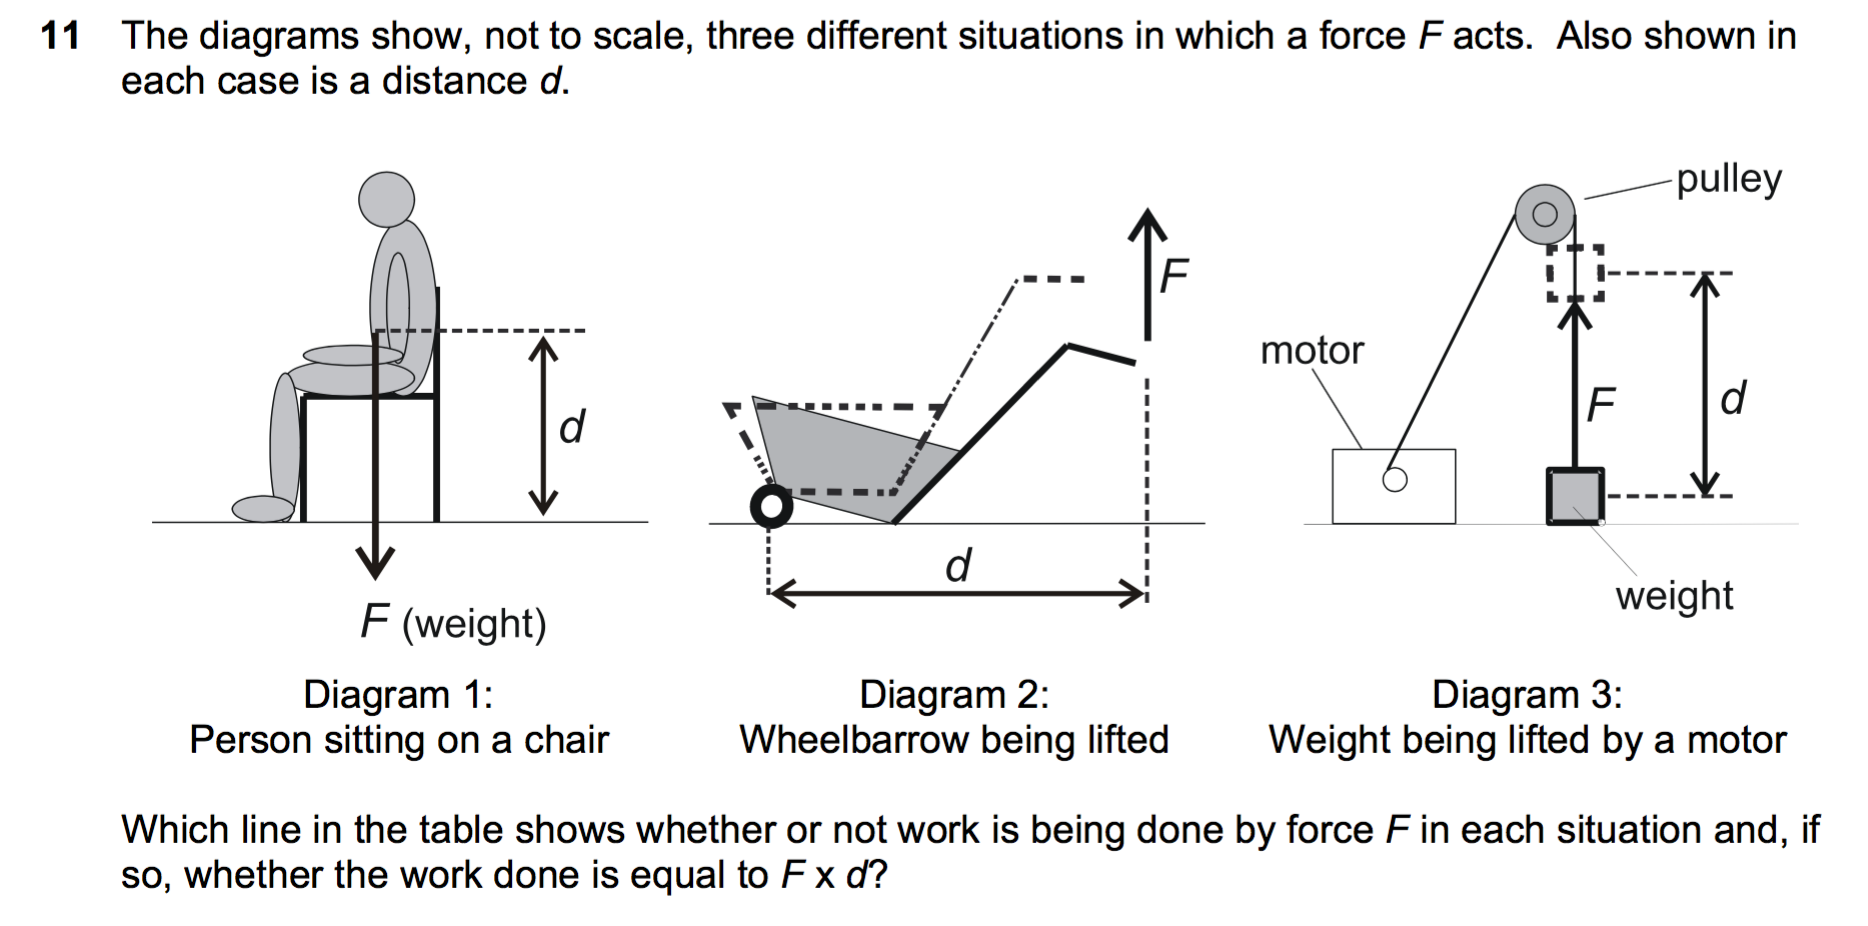
\includegraphics[width=\textwidth]{2012q11}

This example showcases one of the common mistakes people can make when attempting questions regarding work.  Just looking at the equation and memorising won't give actual understanding of the underlying physics.  When calculating the work done by a force, the distance, $d$, is always in the same direction the force is acting.  

Clearly the example with the wheelbarrow does have work being done, as the wheelbarrow isn't moving, but since the distance, $d$, given isn't in the same direction as the force then it's not equal to $F \times d$.  The example of a man sitting on a chair has no work being done, as via Newton's third law he will have an equal and opposite force acted on him by the chair, meaning he isn't moving and resultant force is 0 N.

The pulley, however, is having work done and can be described by $F \times d$ as it is in the same direction as the force.

\section{Thermal Physics}
Thermal physics is a way to describe the effects thermal energy can have upon a system.  Typically this is done using statistics but the basics are easily understood without this.

Most materials can be organised into three separate phases.
\begin{itemize}
\item \textbf{solids}
\item \textbf{liquids}
\item \textbf{gases}
\end{itemize}

Solids are made up of tightly packed atoms bonded together with the important factor being that they do not move from their position.

Liquids on the other hand are randomly arranged and can move around each other as they are bonded together but far more weakly.  This is why water flows and allows other objects to move through it.

Gases are very far apart and move very quickly and randomly.  Since there are no bonds between gas molecules, they are free to move around.

Given enough energy these three states can transform between each other, with the order of increasing energy being solid $\rightarrow$ liquid $\rightarrow$ gas.  As the amount of energy input into the system increases, the temperature increasing, this gives the atoms enough energy to break free of their bonds.  Some good examples of state changes would be candle wax melting into a liquid, water vapour forming around hot water (evaporation) or water freezing into ice at cooler temperatures.

Each state will consequently have different densities, where the density of a system is mass$\div$volume and this is typically in order of decreasing density solid $\rightarrow$ liquid $\rightarrow$ gas (Water and Ice are actually one interesting anomaly to this pattern, due to the complex nature of the bonds).

We can determine different densities by measuring the mass and volume of an object separately, or use Archimedes' principle which involves submerging an object in water and measuring how much water is displaced, with the density of water being a known constant.


Now we need to approach understanding of how thermal energy can transfer through these three states.  There are three ways in which heat can transfer through a system:
\begin{itemize}
\item \textbf{Conduction}
\item \textbf{Convection}
\item \textbf{Radiation}
\end{itemize} 

\subsection{Conduction}
Conduction is the thermal transfer of energy when atoms collide with each other.  Imagine a solid, made up of millions of individual particles.  A particle on the edge gains a large amount of thermal energy, causing it to move as the thermal energy becomes kinetic, resulting in it colliding with all neighbouring particles.  This in turn transfers energy throughout the material as each individual particle gains some of this thermal energy.

If you're applying a constant heat source, you can see how this energy becomes transferred through the system.  Different materials will transfer this heat at different rates due to thermal conductivity.  Metal, as you may have experienced, conducts heat very well.  Air, on the other hand, is a very poor thermal conductor (an insulator) due to how far apart the atoms are in air.

A number of factors affect heat conduction, such as the \textbf{difference in temperature}.  Heat will transfer much faster to a colder area, with speed increasing the further apart their temperatures are.  The \textbf{length} of the object also has an effect as heat has to travel further.  Further, increasing the \textbf{cross-sectional area} of the material will slow the heat transfer. 

\subsection{Convection}
The difference between convection and conduction is that in conduction, the mass contained doesn't move as a whole, whereas convection is heat transfer via mass motion in either a gas or a liquid.  

As a material heats, it becomes less dense as the atoms move apart and therefore will rise (this is why hot air rises).  This is due to the ideal gas law
\begin{equation}
PV = nRT,
\end{equation}
where $P$ is pressure, $V$ is volume, $T$ is temperature, $n$ is the amount of atoms present and $R$ is a constant.  Increasing temperature has to lead to an increase in volume at a constant pressure.

The hot air rises, and the cooler air will drop to replace the warm air that's risen.  This can lead to a circulation of air, as the air will rise, cool down and drop to be replaced by the newer heated air close to the warm source.


\subsection{Radiation}
This is the third form of heat transfer and unlike the previous, requires no mass to transfer the energy.  This heat is transferred via electromagnetic waves, which will be covered in more detail in the next section.  Bodies with a lot of energy will radiate these waves in all directions and will be absorbed by atoms to transfer the energy.  A good example of this type of transfer would be the sun, which transfers all it's heat to us through radiation.

Factors affecting the transfer of radiation will depend on the medium it's travelling through (heat travelling through the atmosphere is absorbed and emitted millions of times on its journey to us), as well as the surface its being absorbed by.  Shiny surfaces are poor at emitting and absorbing, whereas black surfaces are good emitters and absorbers.  The surface area of the material will also greatly affect the rate of absorption and emission




\section{Waves}
The simplest way to view a wave is that it's the transfer of energy through some medium without that medium moving overall from it's original position.  An example might be ripples in water.  The overall body of water isn't moving to carry the energy, but energy is being transferred through it, which you can see.

There are a few concepts you need to know when dealing with waves which are amplitude, frequency, period and wavelength.

A length of a wave over one full oscillation is known as the \textbf{wavelength} or $\mathbf{\lambda}$ as it will be referred to ocassionally.  A full oscillation includes a peak and a trough but effectively it is the smallest repeating unit of the wave.  If you were to take a portion of the wave on a diagram, and copy and paste it infinitely on each end without it changing the shape, then that is the full oscillation.

The \textbf{period} will be the time taken for one whole oscillation to pass a point.

The \textbf{frequency} describes how many full oscillations pass a point in one second (or minute, or hour depending on your units).  Therefore it is the reciprocal of the period, or
\begin{equation*}
\mathbf{f = \frac{1}{t}}.
\end{equation*}

The \textbf{amplitude} is the height of the wave's oscillations from the origin.

\begin{figure}[H]
\centering
% This file was created by matplotlib2tikz v0.5.7.
% The lastest updates can be retrieved from
% 
% https://github.com/nschloe/matplotlib2tikz
% 
% where you can also submit bug reports and leavecomments.
% 
\begin{tikzpicture}

\begin{axis}[
hide x axis,
hide y axis,
xmin=0, xmax=6.28318530717959,
ymin=-1.5, ymax=1.5,
axis on top
]
\addplot [red]
table {%
0 0
0.0634665182543393 0.0634239196565645
0.126933036508679 0.126592453573749
0.190399554763018 0.18925124436041
0.253866073017357 0.251147987181079
0.317332591271696 0.312033445698487
0.380799109526036 0.371662455660328
0.444265627780375 0.429794912089172
0.507732146034714 0.486196736100469
0.571198664289053 0.540640817455598
0.634665182543393 0.59290792905464
0.698131700797732 0.642787609686539
0.761598219052071 0.690079011482112
0.82506473730641 0.734591708657533
0.88853125556075 0.776146464291757
0.951997773815089 0.814575952050336
1.01546429206943 0.849725429949514
1.07893081032377 0.881453363447582
1.14239732857811 0.909631995354518
1.20586384683245 0.934147860265107
1.26933036508679 0.954902241444074
1.33279688334112 0.971811568323542
1.39626340159546 0.984807753012208
1.4597299198498 0.993838464461254
1.52319643810414 0.998867339183008
1.58666295635848 0.999874127673875
1.65012947461282 0.996854775951942
1.71359599286716 0.989821441880933
1.7770625111215 0.978802446214779
1.84052902937584 0.963842158559942
1.90399554763018 0.945000818714668
1.96746206588452 0.922354294104581
2.03092858413886 0.895993774291336
2.0943951023932 0.866025403784439
2.15786162064753 0.832569854634771
2.22132813890187 0.795761840530832
2.28479465715621 0.755749574354258
2.34826117541055 0.712694171378863
2.41172769366489 0.666769000516292
2.47519421191923 0.618158986220605
2.53866073017357 0.567059863862771
2.60212724842791 0.513677391573406
2.66559376668225 0.458226521727411
2.72906028493659 0.400930535406614
2.79252680319093 0.342020143325669
2.85599332144527 0.28173255684143
2.91945983969961 0.220310532786541
2.98292635795395 0.15800139597335
3.04639287620828 0.0950560433041824
3.10985939446262 0.0317279334980677
3.17332591271696 -0.0317279334980679
3.2367924309713 -0.0950560433041826
3.30025894922564 -0.15800139597335
3.36372546747998 -0.220310532786541
3.42719198573432 -0.28173255684143
3.49065850398866 -0.342020143325669
3.554125022243 -0.400930535406614
3.61759154049734 -0.45822652172741
3.68105805875168 -0.513677391573406
3.74452457700602 -0.567059863862771
3.80799109526036 -0.618158986220605
3.87145761351469 -0.666769000516292
3.93492413176903 -0.712694171378863
3.99839065002337 -0.755749574354258
4.06185716827771 -0.795761840530832
4.12532368653205 -0.832569854634771
4.18879020478639 -0.866025403784439
4.25225672304073 -0.895993774291336
4.31572324129507 -0.922354294104581
4.37918975954941 -0.945000818714668
4.44265627780375 -0.963842158559942
4.50612279605809 -0.978802446214779
4.56958931431243 -0.989821441880933
4.63305583256677 -0.996854775951942
4.69652235082111 -0.999874127673875
4.75998886907544 -0.998867339183008
4.82345538732978 -0.993838464461254
4.88692190558412 -0.984807753012208
4.95038842383846 -0.971811568323542
5.0138549420928 -0.954902241444074
5.07732146034714 -0.934147860265107
5.14078797860148 -0.909631995354518
5.20425449685582 -0.881453363447582
5.26772101511016 -0.849725429949514
5.3311875333645 -0.814575952050336
5.39465405161884 -0.776146464291757
5.45812056987318 -0.734591708657533
5.52158708812752 -0.690079011482112
5.58505360638185 -0.64278760968654
5.64852012463619 -0.59290792905464
5.71198664289053 -0.540640817455597
5.77545316114487 -0.486196736100469
5.83891967939921 -0.429794912089172
5.90238619765355 -0.371662455660327
5.96585271590789 -0.312033445698487
6.02931923416223 -0.251147987181079
6.09278575241657 -0.18925124436041
6.15625227067091 -0.126592453573749
6.21971878892525 -0.0634239196565645
6.28318530717959 -2.44929359829471e-16
};
\draw[<->,black] (axis cs:1.5707963267949,0) -- (axis cs:1.5707963267949,1);
\node at (axis cs:1.5707963267949,0)[
  scale=0.6,
  anchor=base west,
  text=black,
  rotate=0.0
]{ };
\draw[<->,black] (axis cs:6.28318530717959,0) -- (axis cs:0,0);
\node at (axis cs:6.28318530717959,0)[
  scale=0.6,
  anchor=base west,
  text=black,
  rotate=0.0
]{ };
\node at (axis cs:4.5,0.1)[
  scale=0.6,
  anchor=base west,
  text=black,
  rotate=0.0
]{ Wavelength};
\node at (axis cs:1.6,0.4)[
  scale=0.6,
  anchor=base west,
  text=black,
  rotate=0.0
]{ Amplitude};
\end{axis}

\end{tikzpicture}
\end{figure}

We can describe the speed of the wave using $v=\frac{d}{t}$ as well, so this in terms of the wave quantities is
\begin{equation}
\mathbf{v = f \times \lambda}.
\end{equation}

There are \textbf{two speeds you are commonly required to know}.

\begin{description}
\item[Sound] Typically 340 m/s
\item[Electromagnetic] $3\times10^8$ m/s.
\end{description}

There are also two types of waves to consider, transverse and longitudinal.  

Transverse waves oscillate perpendicular to the actual energy movement.  An example of these would be light waves.  As shown here the direction of movement is perpendicular to that of oscillation.
\begin{figure}[H]
\centering
% This file was created by matplotlib2tikz v0.5.7.
% The lastest updates can be retrieved from
% 
% https://github.com/nschloe/matplotlib2tikz
% 
% where you can also submit bug reports and leavecomments.
% 
\begin{tikzpicture}

\begin{axis}[
hide x axis,
hide y axis,
xmin=0, xmax=10,
ymin=-1.5, ymax=1.5,
axis on top
]
\addplot [red]
table {%
0 0
0.101010101010101 0.100838420258105
0.202020202020202 0.200648856522685
0.303030303030303 0.298413804447641
0.404040404040404 0.39313661214833
0.505050505050505 0.483851640437935
0.606060606060606 0.569634106908966
0.707070707070707 0.649609513505707
0.808080808080808 0.72296256147946
0.909090909090909 0.788945462844257
1.01010101010101 0.846885563602983
1.11111111111111 0.896192201029956
1.21212121212121 0.936362725104285
1.31313131313131 0.9669876227093
1.41414141414141 0.987754692360084
1.51515151515152 0.998452226900389
1.61616161616162 0.998971171723357
1.71717171717172 0.98930623651434
1.81818181818182 0.969555949182324
1.91919191919192 0.939921651430131
2.02020202020202 0.900705446202955
2.12121212121212 0.852307117939675
2.22222222222222 0.795220057023049
2.32323232323232 0.730026229976446
2.42424242424242 0.657390246682775
2.52525252525253 0.578052585106573
2.62626262626263 0.492822042588923
2.72727272727273 0.402567490669497
2.82828282828283 0.308209017490077
2.92929292929293 0.210708548077193
3.03030303030303 0.11106003812413
3.13131313131313 0.0102793412405347
3.23232323232323 -0.0906061470334077
3.33333333333333 -0.190567962875485
3.43434343434343 -0.288587058720432
3.53535353535354 -0.383664191806112
3.63636363636364 -0.47483011082224
3.73737373737374 -0.561155436815202
3.83838383838384 -0.641760137619388
3.93939393939394 -0.71582249922919
4.04040404040404 -0.782587502654202
4.14141414141414 -0.84137452086087
4.24242424242424 -0.89158425733514
4.34343434343434 -0.932704855531834
4.44444444444444 -0.964317116928778
4.54545454545454 -0.98609877449093
4.64646464646465 -0.997827777979213
4.74747474747475 -0.999384557612436
4.84848484848485 -0.990753243005677
4.94949494949495 -0.972021824958833
5.05050505050505 -0.943381258446
5.15151515151515 -0.905123515950137
5.25252525252525 -0.857638610988052
5.35353535353535 -0.80141062216897
5.45454545454545 -0.737012758318913
5.55555555555556 -0.665101514978822
5.65656565656566 -0.586409981847235
5.75757575757576 -0.501740369393911
5.85858585858586 -0.411955830830863
5.95959595959596 -0.317971662810619
6.06060606060606 -0.220745974555063
6.16161616161616 -0.121269920537167
6.26262626262626 -0.0205575962872601
6.36363636363636 0.0803642996702817
6.46464646464646 0.180466932359911
6.56565656565657 0.278729818677557
6.66666666666667 0.37415123057122
6.76767676767677 0.465758407025652
6.86868686868687 0.552617470746406
6.96969696969697 0.633842948448906
7.07070707070707 0.708606797699218
7.17171717171717 0.77614684828358
7.27272727272727 0.835774572052259
7.37373737373737 0.886882102029079
7.47474747474747 0.928948429231251
7.57575757575758 0.961544714026824
7.67676767676768 0.984338657883824
7.77777777777778 0.997097890943875
7.87878787878788 0.999692340886112
7.97979797979798 0.992095558932323
8.08080808080808 0.974384989475536
8.18181818181818 0.946741180583354
8.28282828282828 0.909445943424463
8.38383838383838 0.862879479381784
8.48484848484848 0.807516504139563
8.58585858585859 0.743921408256844
8.68686868686869 0.672742503562265
8.78787878787879 0.594705414024497
8.88888888888889 0.510605678474283
8.98989898989899 0.421300640588607
9.09090909090909 0.3277007088135
9.19191919191919 0.230760075325052
9.29292929292929 0.131466988642958
9.39393939393939 0.030833679061141
9.49494949494949 -0.0701139604006468
9.5959595959596 -0.170346832328096
9.6969696969697 -0.268843125910384
9.7979797979798 -0.364598733655889
9.8989898989899 -0.456637487633774
10 -0.54402111088937
};
\path [draw=black, fill=black] (axis cs:4.3,1.2)
--(axis cs:4.2,1.175)
--(axis cs:4.2,1.1995)
--(axis cs:0.200000000000001,1.1995)
--(axis cs:0.200000000000001,1.2005)
--(axis cs:4.2,1.2005)
--(axis cs:4.2,1.225)
--cycle;

\end{axis}

\end{tikzpicture}
\end{figure}

Longitudinal however, will oscillate in the same direction of motion, which are a little difficult to visualise.  These include sound waves and seismic waves, but typically when actually drawing these they can be treated with the same equations and thus will be drawn similarly.



\subsection{Behaviour}
Waves have different behaviours when passing through different mediums.

Reflection occurs when the wave meets a boundary, and will reflect at an angle equal to that it met the boundary at, the angle of incidence.  The normal in this example is an imaginary line that cuts perpendicularly through the boundary.

\begin{figure}[H]
\centering
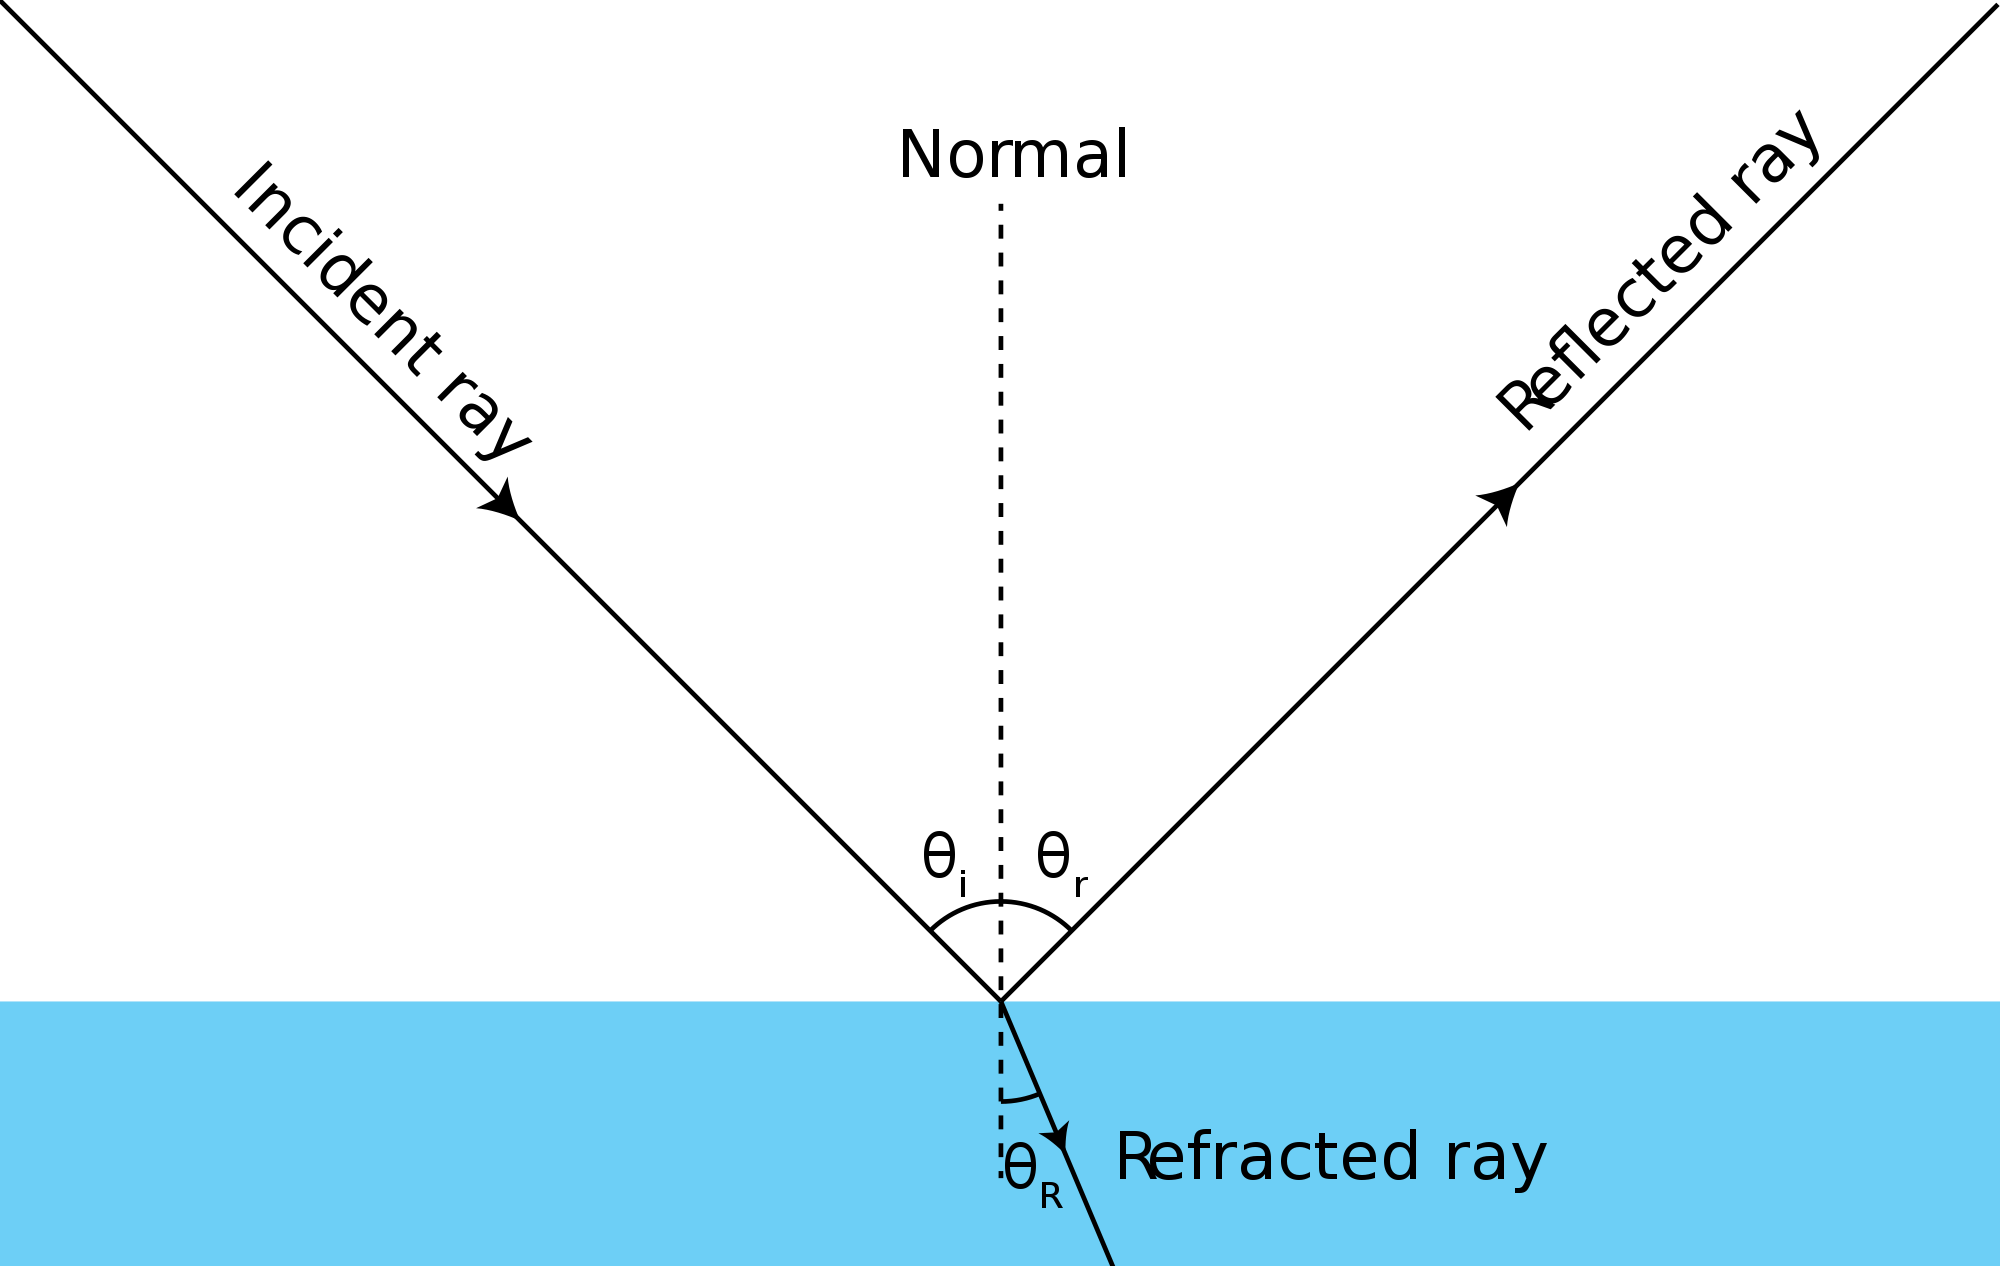
\includegraphics[width=0.8\textwidth]{incidence-reflection}
\end{figure}

Refraction occurs when a wave meets a medium with a different density to the one it was passing through.  If the density of the medium is higher then the light wave will speed up and pass through at a closer angle to the normal, e.g. $\theta_R < \theta_i$.  If it's a lower density then the angle will be greater than the incident angle.

At a planar boundary, a flat surface, where only reflection will happen, \textbf{the angle of incidence is equal to the angle of reflection.}

\subsubsection*{Total Internal Reflection}
This has come up before so its important to cover it.  If going from a \textbf{more dense material to a less dense one}, the wave will speed up, but if the angle of incidence is \textbf{greater than a certain critical angle} then the wave can reflect back into the original material instead of refracting.

Both criteria have to be fulfilled for total internal reflection to occur. 

\subsubsection*{Example}

\begin{figure}[H]
\centering
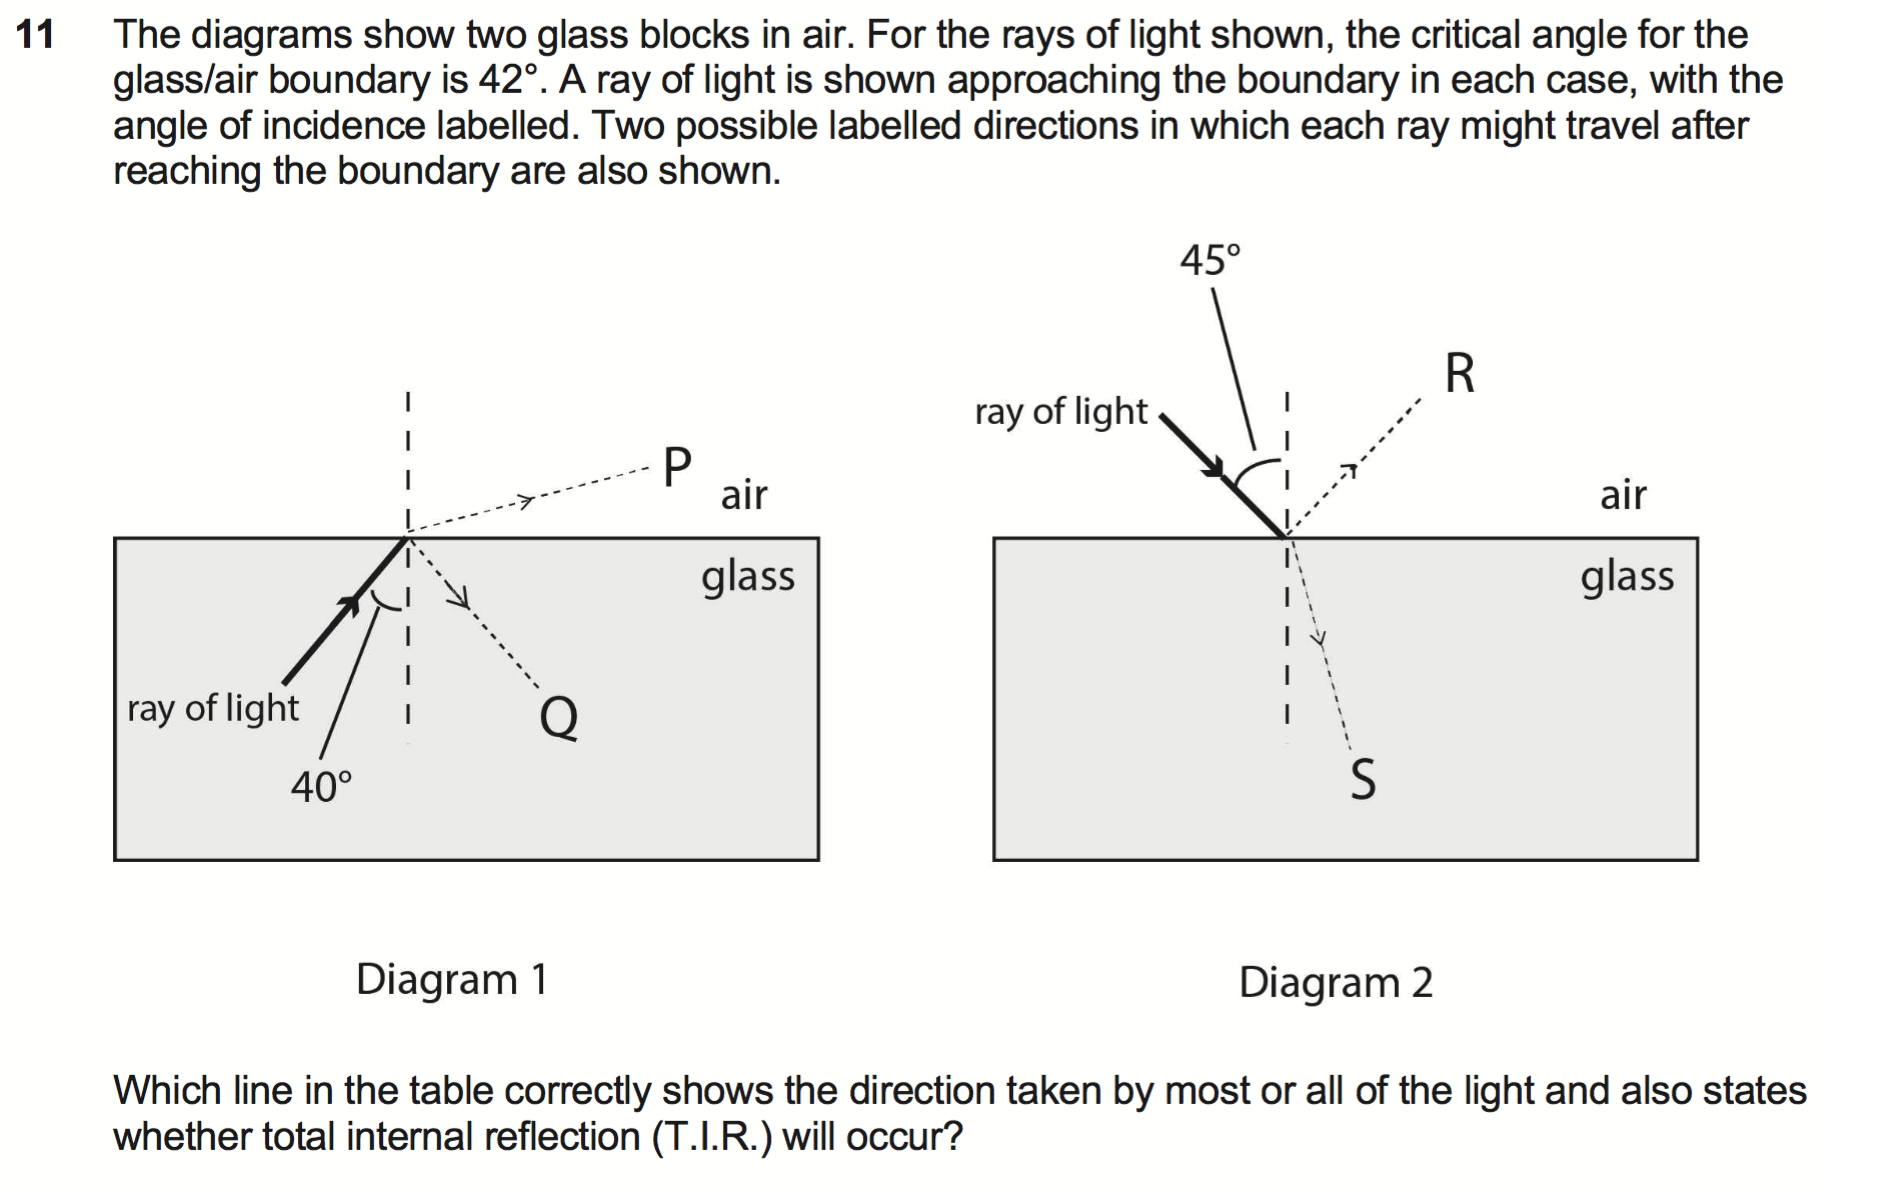
\includegraphics[width=\textwidth]{2013q11}
\end{figure}

For the first diagram, we've been told that the incident angle is $40^\circ$ which is lower than the critical angle indicating that the ray will follow path P.  Therefore no internal reflection.

For the second diagram, the ray is travelling from air to glass, less dense to more dense, so internal reflection cannot occur anyway and the ray will follow path S.

\subsubsection*{The Doppler Effect}
One other effect that must be mentioned is the doppler effect.  If you've ever heard a police car or ambulance passing you, you've experienced the doppler effect.  

As it approaches, it sounds much higher than it does after it's passed and is moving away.  This is because as it's approaching, each wave peak will be much closer to the previous one, effectively it's frequency has been increased because the object is moving. 

Conversely, the reverse is also true as it recedes, as the next peak will be farther away than the previous one, reducing it's frequency.  


\subsection{Sound Waves}
A quick overview of sound waves also has to be covered so that you're aware of their unique properties.  Firstly, they are longitudinal waves, which as discussed means they oscillate in the same direction of propagation.

They will behave in the same manner as other types of waves, but one interesting phenomena is that of echoes, which is the sound wave reflecting off the environment.

Sound waves have a number of applications in frequencies above that which we can audibly hear, known as ultrasound.  The high frequency waves are reflected off objects and the time for them to return allows us to calculate where certain objects may be.  This is how sonar, medical ultrasound (seeing inside the womb for example) and deep sea scanning work.


\subsection{Modelling Real Physical Systems}
Hopefully, by now you should have a decent grasp of how waves work and the necessary equations, but in a large number of questions you'll have to apply them to an actual physical system.  In some cases this is obvious as we're dealing with actual waves, but in others its not quite as easy.  Lets look at a quick example. 

\subsection*{Example 1}

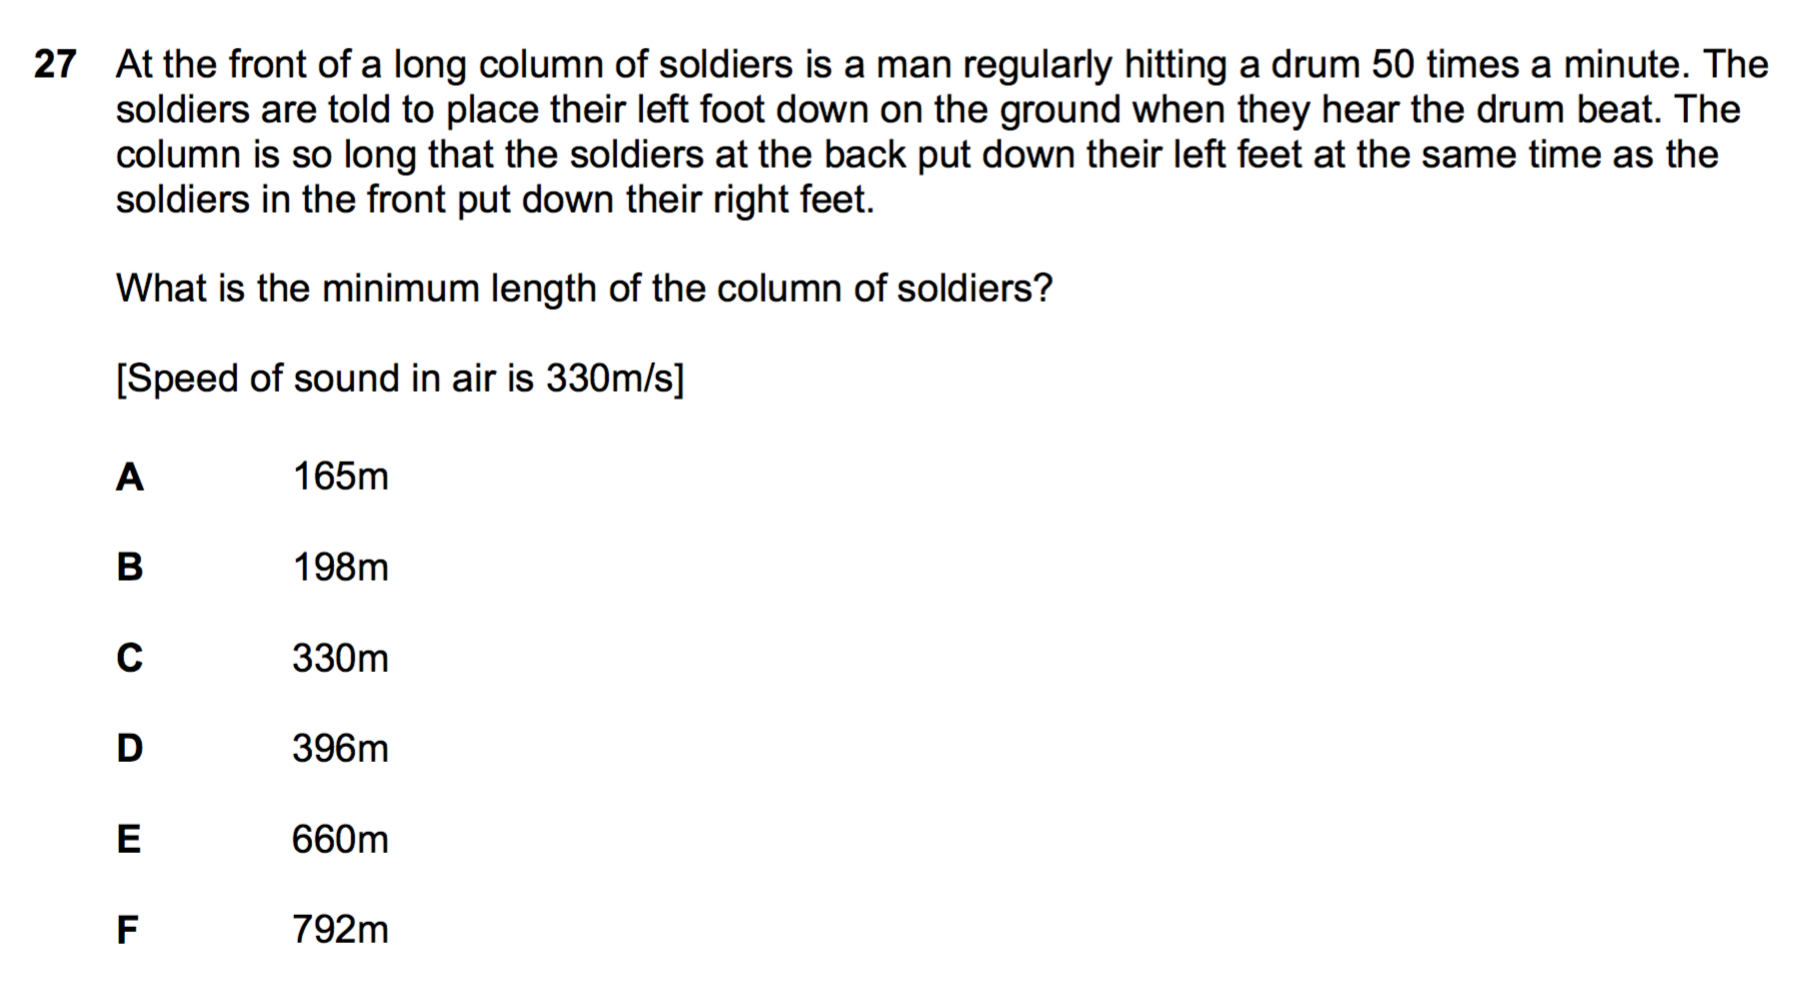
\includegraphics[width=\textwidth]{2011q27}

This is from the 2011 paper and don't worry if how to approach this isn't too obvious.  

Firstly, look for information in the question that applies to the equations that you already know.  The man at the front beats the drum 50 times a minute.  They've given us a result for the frequency with which he hits the drum and we're also given the speed of sound.  So how does this relate to the length of the column?

Going back to the question, we know that the soldier at the front puts his right foot down as the one at the back puts down his left foot and vice versa.  This motion is very similar to a wave, the right foot movement representing a peak and the left foot a trough.  Modelling it in this way, the total length of soldiers is effectively half of a total wavelength.  

Then tackling the question is simply a matter of $v=f \lambda$ and dividing the result for $\lambda$ by 2 to get the column length.  

\subsection*{Example 2}

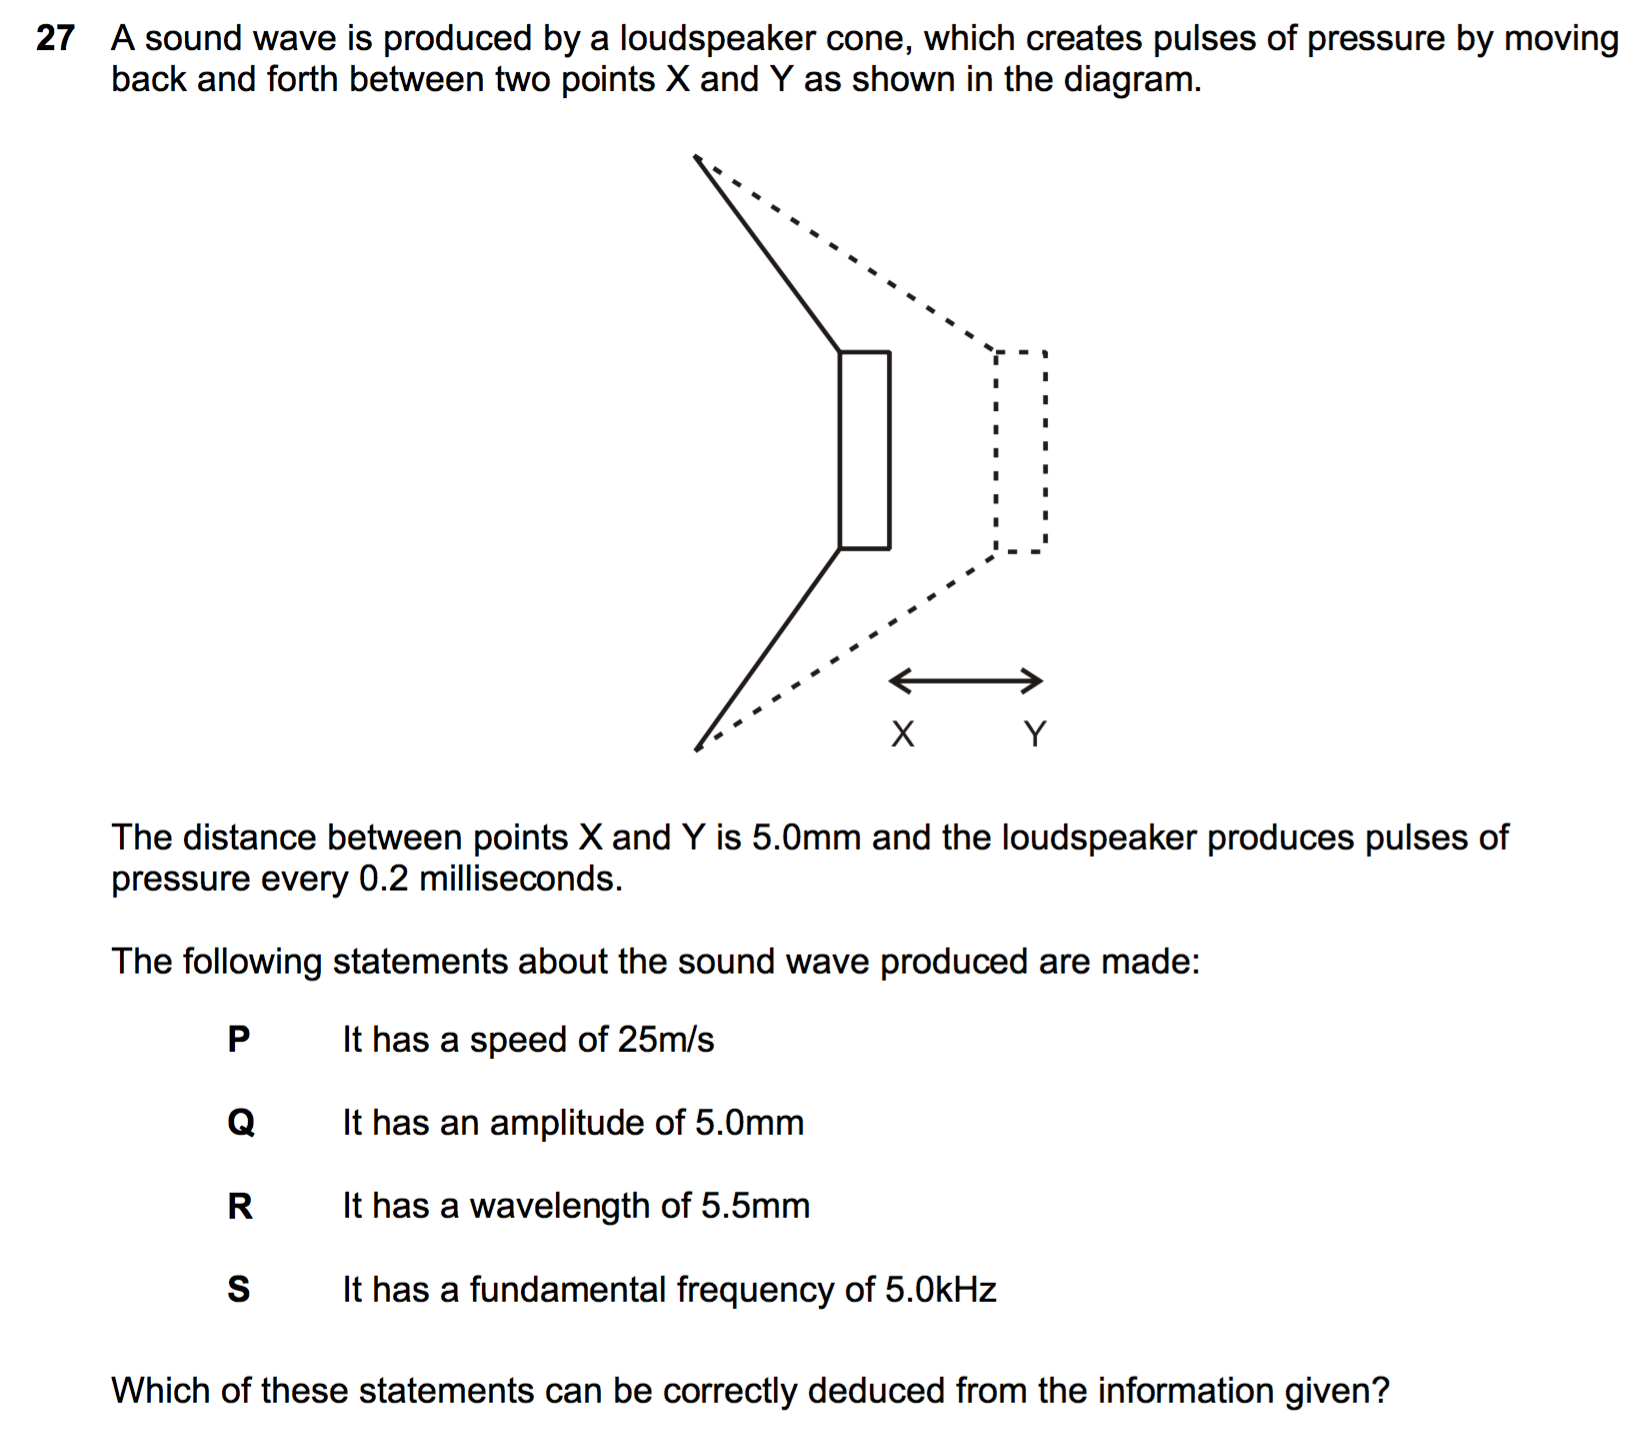
\includegraphics[width=\textwidth]{2012q27}

This is the same kind of situation, find ways to apply the equations you know to what you've been given.  We know the distance the speaker oscillates over, and if we model this motion as a wave we see the distance $\textbf{XY}$, will be twice the amplitude of a wave.  Since it produces pulses of pressure every 0.2 milliseconds we can calculate the frequency also.  From this all the information we need is available.


\section{EM Waves}
We've covered the fundamentals of waves, but one of the most important types are those in the electromagnetic spectrum.  This includes radio, visible light and a host of other types.  These are transverse and propagate through a vacuum at the speed of light.  In air or water they will propagate slower due to absorption and re-emission but this is unlikely to be something they will test.  The full spectrum is included here from lowest energy to highest energy.
\begin{table}[H]
\centering
\begin{tabular}{c|ccccc}
&Wavelength & Frequency (Hz)\\
\hline
Radio Waves & >10cm &$<3\times10^7$\\
Microwaves&1mm - 10cm & $3\times10^9$ - $3\times10^{11}$\\
Infrared&30mm - 1mm &$3\times10^{11}$ - $4\times10^{14}$\\
Visible Light&400nm - 700nm & $4\times10^{14}$ - $7\times10^{14}$\\
Ultra-Violet&10nm - 400 nm & $7\times10^{14}$ - $3\times10^{16}$\\
X-Rays&0.01nm - 10nm & $3\times10^{16}$ - $3\times10^{19}$\\
Gamma&<0.01nm & $>3\times10^{19}$\\
\end{tabular}
\caption*{Source: https://www.pa.msu.edu/courses/2000fall/PHY232/lectures/emwaves/spectrum.html}
\end{table}

These definitions are quite fluid and there will be different sources giving different values, but they key here is that they will be of the same order of magnitude.  The important thing here is not to memorise exactly the different frequencies but you should be able to ballpark each of the wavelengths and be able to order them correctly in decreasing wavelength/frequency/energy.

\subsection{Uses}
Each of these parts of the spectrum has their own uses and dangers.  It's very important that you are able to correctly identify these.

\subsubsection*{Radio}
Radio waves are most commonly used in radio communication or broadcasting.  There are very few to no dangers associated with these waves due to their lower energy.

\subsubsection*{Microwaves}
These are used in cooking as they can be absorbed by water molecules, or also in communication with satellites or mobile calls.  A poor microwave oven may disrupt these signals for this reason.  

The main danger associated with microwaves is damage to cells as water molecules heat up when absorbing them.  This requires a very high dose to cause damage however.

\subsubsection*{Infrared}
This is what we commonly associate with heat as it is absorbed and emitted by the skin.  Mostly this is used in heating appliances like toasters or heaters.

\subsubsection*{Visible Light}
This is the light you see.  There are very few dangers associated with this form of light.

\subsubsection*{Ultraviolet}
A large amount of this form of light is emitted by the sun and is commonly used in tanning beds as this causes our skin to become darker.  However, it has the potential to cause skin damage and can cause cells to become cancerous.

\subsubsection*{X-Rays}
Used to visualise parts of the body or used as part of security scanners.  This form of EM waves is dangerous as it has a high penetrative power and can ionise cells causing them to become cancerous.  The number of X-rays you have is consequently monitored to reduce the risk of you receiving a damaging dose.

\subsubsection*{Gamma Rays}
These are used most commonly to sterilise surgical equipment or kill bacteria in food.  They are highly energetic and very dangerous having the potential to be fatal in high enough doses, or cause cancer in lower doses.

\section{Radioactivity}
This section deals with the structure of atoms.  You should already have an understanding of how molecules and atoms move in different physical states (gas, liquid or solid) but now we're going to look at what makes up these atoms.

Firstly, all atoms are made up of three components,
\begin{description}
\item[Electrons] Negative charge, mass of $9.1\times10^{-31}$kg.
\item[Protons] Positive charge, mass of $1.7\times10^{-27}$kg.
\item[Neutrons] Neutral charge, mass of  $1.7\times10^{-27}$kg.
\end{description}

Atoms are formed of a nucleus comprised of neutrons and protons bonded together.  Orbiting this nucleus are electron as illustrated.  
\begin{figure}[H]
\centering
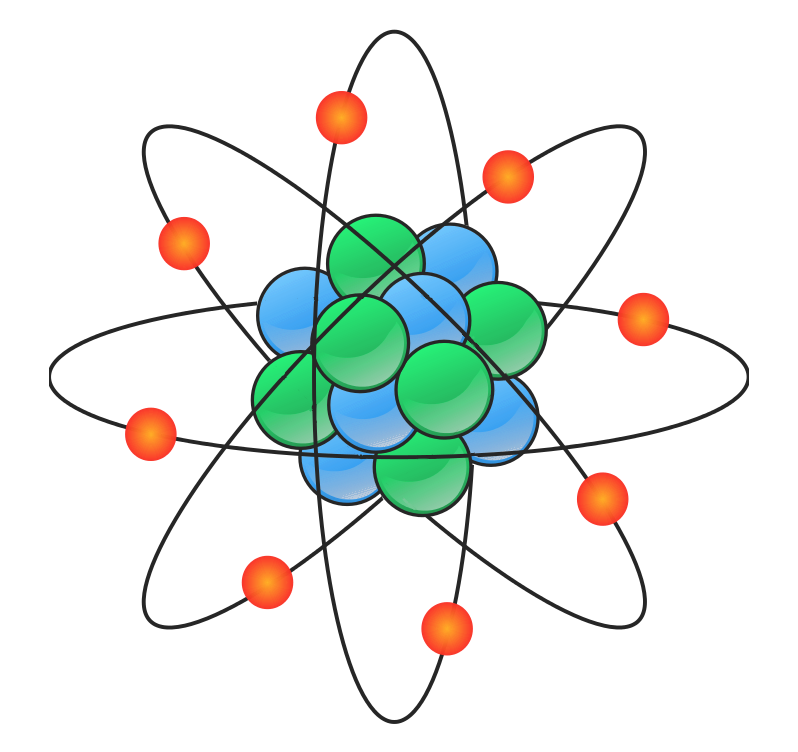
\includegraphics[width=0.5\textwidth]{atom}
\end{figure}


In a neutral atom, the number of protons will be equal to the number of electrons as they have exactly equal but opposite charges.  Remove an electron, or remove a proton and the atom becomes \textbf{ionised}: it now carries a charge.

We denote most chemical symbols via this notation
{\Large\ce{^{M}_{P}X}}.

In place of \textbf{M}, the mass number, we note the number of protons added to the number of neutrons.  \textbf{P} is the proton number and we note the number of protons there.  In place of X we put chemical symbol, for example $H$ if we were dealing with hydrogen.

An example of this could be Carbon.  We denote it as 
{\Large{\ce{^{12}_{6}C}}},
but if we were to remove an electron, ionising it, we form
{{\Large{\ce{^{12}_{5}C^+}}}}.

The different types of atoms, Carbon, Hydrogen, etc. are dependent upon the number of protons in the nucleus.  This will have the largest effect on the chemical expression of the atom.  We can also form different stable \textbf{isotopes} which are atoms with the same number of electrons and protons but different mass numbers, these will not behave very differently.


\subsection{Decay}
Atoms are not completely stable and can undergo different forms of decay transforming into various other atoms or ions.  The three types of radiation are alpha, beta and gamma. 

 

\subsubsection*{Alpha}
Alpha radiation is formed from a Helium nucleus breaking free from the atom, {{\Large{\ce{^{4}_{2}He}}}}.  In this type of decay we reduce the mass number of the original atom by 4, and it's proton number by 2.

Alpha radiation cannot penetrate paper and cannot move more than around 5cm through air.  They are highly ionising however, and if a source is ingested it can do a tremendous amount of damage

\subsubsection*{Beta}
Beta decay is the expulsion of an electron from the nucleus of the atom.  Its important to note that the atom doesn't lose any orbiting electrons.

A neutron can decay into a proton, and since we need to conserve charge, this decay results in an electron being expelled.  There are no changes to the mass number in this case, but the proton number does increase by 1.

Beta radiation can penetrate anything up to a thick sheet of aluminium and can move around 15cm through air.  They are fairly ionising but are not likely to come in contact with an atom due to the small size of the electron.

\subsubsection*{Gamma}
If the nucleus is unstable, it may emit gamma rays which will stabilise the nucleus slightly.  This has no effect upon the mass, charge or proton numbers.
Gamma rays are highly penetrative, highly ionising and very long range.


There are low levels of radiation all around us in what is known as background radiation.  This can come from rocks and all manner of minerals, cosmic rays or even plants.  Also artificial sources such as radioactive waste and medical x-rays will add to the background radiation.  Luckily the background is low enough to not cause us a big risk yet.



\subsection{Half-Life}
We define the activity of a sample as how many decays it undergoes in a certain amount of time.  Of course over time this will decrease as the sample stabilises, but this will happen exponentially, there will be no set time when radioactivity will end.  Consequently, we use the term half-life to describe the rate at which a sample's decay rate ceases.  

The half-life is the time taken for the sample's activity to halve.  Say we have a half-life of 1 minute and an initial activity of 100.  In 1 minute it will be 50, after another 1 it will be 25 and so on.  We can visualise this thusly.
  
\begin{figure}[H]
\centering
% This file was created by matplotlib2tikz v0.5.7.
% The lastest updates can be retrieved from
% 
% https://github.com/nschloe/matplotlib2tikz
% 
% where you can also submit bug reports and leavecomments.
% 
\begin{tikzpicture}

\begin{axis}[
xlabel={Time (s)},
ylabel={Activity},
xmin=0, xmax=4,
ymin=0, ymax=100,
axis on top
]
\addplot [red]
table {%
0 100
0.01 99.3092495437036
0.02 98.6232704493359
0.03 97.9420297586927
0.04 97.2654947412286
0.05 96.5936328924846
0.06 95.9264119325264
0.07 95.2637998043937
0.08 94.6057646725596
0.09 93.9522749214012
0.1 93.3032991536807
0.11 92.6588061890371
0.12 92.0187650624875
0.13 91.3831450229401
0.14 90.7519155317161
0.15 90.125046261083
0.16 89.5025070927972
0.17 88.884268116657
0.18 88.2702996290655
0.19 87.6605721316035
0.2 87.0550563296124
0.21 86.4537231307865
0.22 85.8565436437754
0.23 85.2634891767957
0.24 84.6745312362527
0.25 84.0896415253714
0.26 83.5087919428369
0.27 82.9319545814442
0.28 82.3591017267573
0.29 81.7902058557781
0.3 81.2252396356236
0.31 80.6641759222126
0.32 80.1069877589622
0.33 79.5536483754919
0.34 79.0041311863377
0.35 78.4584097896751
0.36 77.91645796605
0.37 77.3782496771195
0.38 76.8437590644006
0.39 76.312960448028
0.4 75.7858283255199
0.41 75.2623373705534
0.42 74.7424624317469
0.43 74.2261785314525
0.44 73.7134608645551
0.45 73.2042847972813
0.46 72.6986258660155
0.47 72.1964597761248
0.48 71.6977624007914
0.49 71.2025097798536
0.5 70.7106781186548
0.51 70.2222437868999
0.52 69.7371833175203
0.53 69.2554734055462
0.54 68.7770909069872
0.55 68.3020128377198
0.56 67.8302163723836
0.57 67.3616788432845
0.58 66.8963777393056
0.59 66.4342907048256
0.6 65.9753955386447
0.61 65.5196701929182
0.62 65.0670927720967
0.63 64.6176415318746
0.64 64.1712948781452
0.65 63.7280313659631
0.66 63.287829698514
0.67 62.8506687260914
0.68 62.4165274450806
0.69 61.9853849969493
0.7 61.5572206672458
0.71 61.1320138846034
0.72 60.7097442197524
0.73 60.290391384538
0.74 59.8739352309464
0.75 59.4603557501361
0.76 59.0496330714765
0.77 58.6417474615939
0.78 58.2366793234228
0.79 57.8344091952644
0.8 57.4349177498517
0.81 57.0381857934212
0.82 56.6441942647899
0.83 56.2529242344405
0.84 55.864356903611
0.85 55.4784736033923
0.86 55.0952557938305
0.87 54.714685063037
0.88 54.3367431263029
0.89 53.9614118252214
0.9 53.5886731268147
0.91 53.218509122668
0.92 52.850902028069
0.93 52.4858341811534
0.94 52.1232880420561
0.95 51.7632461920689
0.96 51.4056913328033
0.97 51.0506062853597
0.98 50.6979739895015
0.99 50.3477775028359
1 50
1.01 49.6546247718518
1.02 49.311635224668
1.03 48.9710148793463
1.04 48.6327473706143
1.05 48.2968164462423
1.06 47.9632059662632
1.07 47.6318999021969
1.08 47.3028823362798
1.09 46.9761374607006
1.1 46.6516495768404
1.11 46.3294030945185
1.12 46.0093825312438
1.13 45.69157251147
1.14 45.375957765858
1.15 45.0625231305415
1.16 44.7512535463986
1.17 44.4421340583285
1.18 44.1351498145327
1.19 43.8302860658018
1.2 43.5275281648062
1.21 43.2268615653933
1.22 42.9282718218877
1.23 42.6317445883978
1.24 42.3372656181264
1.25 42.0448207626857
1.26 41.7543959714185
1.27 41.4659772907221
1.28 41.1795508633787
1.29 40.8951029278891
1.3 40.6126198178118
1.31 40.3320879611063
1.32 40.0534938794811
1.33 39.7768241877459
1.34 39.5020655931689
1.35 39.2292048948375
1.36 38.958228983025
1.37 38.6891248385597
1.38 38.4218795322003
1.39 38.156480224014
1.4 37.89291416276
1.41 37.6311686852767
1.42 37.3712312158735
1.43 37.1130892657262
1.44 36.8567304322775
1.45 36.6021423986406
1.46 36.3493129330078
1.47 36.0982298880624
1.48 35.8488812003957
1.49 35.6012548899268
1.5 35.3553390593274
1.51 35.1111218934499
1.52 34.8685916587601
1.53 34.6277367027731
1.54 34.3885454534936
1.55 34.1510064188599
1.56 33.9151081861918
1.57 33.6808394216423
1.58 33.4481888696528
1.59 33.2171453524128
1.6 32.9876977693224
1.61 32.7598350964591
1.62 32.5335463860483
1.63 32.3088207659373
1.64 32.0856474390726
1.65 31.8640156829815
1.66 31.643914849257
1.67 31.4253343630457
1.68 31.2082637225403
1.69 30.9926924984747
1.7 30.7786103336229
1.71 30.5660069423017
1.72 30.3548721098762
1.73 30.145195692269
1.74 29.9369676154732
1.75 29.730177875068
1.76 29.5248165357383
1.77 29.320873730797
1.78 29.1183396617114
1.79 28.9172045976322
1.8 28.7174588749259
1.81 28.5190928967106
1.82 28.322097132395
1.83 28.1264621172202
1.84 27.9321784518055
1.85 27.7392368016961
1.86 27.5476278969153
1.87 27.3573425315185
1.88 27.1683715631514
1.89 26.9807059126107
1.9 26.7943365634073
1.91 26.609254561334
1.92 26.4254510140345
1.93 26.2429170905767
1.94 26.061644021028
1.95 25.8816230960344
1.96 25.7028456664017
1.97 25.5253031426798
1.98 25.3489869947507
1.99 25.173888751418
2 25
2.01 24.8273123859259
2.02 24.655817612334
2.03 24.4855074396732
2.04 24.3163736853071
2.05 24.1484082231211
2.06 23.9816029831316
2.07 23.8159499510984
2.08 23.6514411681399
2.09 23.4880687303503
2.1 23.3258247884202
2.11 23.1647015472593
2.12 23.0046912656219
2.13 22.845786255735
2.14 22.687978882929
2.15 22.5312615652708
2.16 22.3756267731993
2.17 22.2210670291643
2.18 22.0675749072664
2.19 21.9151430329009
2.2 21.7637640824031
2.21 21.6134307826966
2.22 21.4641359109438
2.23 21.3158722941989
2.24 21.1686328090632
2.25 21.0224103813429
2.26 20.8771979857092
2.27 20.732988645361
2.28 20.5897754316893
2.29 20.4475514639445
2.3 20.3063099089059
2.31 20.1660439805532
2.32 20.0267469397406
2.33 19.888412093873
2.34 19.7510327965844
2.35 19.6146024474188
2.36 19.4791144915125
2.37 19.3445624192799
2.38 19.2109397661002
2.39 19.078240112007
2.4 18.94645708138
2.41 18.8155843426383
2.42 18.6856156079367
2.43 18.5565446328631
2.44 18.4283652161388
2.45 18.3010711993203
2.46 18.1746564665039
2.47 18.0491149440312
2.48 17.9244406001978
2.49 17.8006274449634
2.5 17.6776695296637
2.51 17.555560946725
2.52 17.4342958293801
2.53 17.3138683513866
2.54 17.1942727267468
2.55 17.0755032094299
2.56 16.9575540930959
2.57 16.8404197108211
2.58 16.7240944348264
2.59 16.6085726762064
2.6 16.4938488846612
2.61 16.3799175482295
2.62 16.2667731930242
2.63 16.1544103829687
2.64 16.0428237195363
2.65 15.9320078414908
2.66 15.8219574246285
2.67 15.7126671815229
2.68 15.6041318612701
2.69 15.4963462492373
2.7 15.3893051668115
2.71 15.2830034711509
2.72 15.1774360549381
2.73 15.0725978461345
2.74 14.9684838077366
2.75 14.865088937534
2.76 14.7624082678691
2.77 14.6604368653985
2.78 14.5591698308557
2.79 14.4586022988161
2.8 14.3587294374629
2.81 14.2595464483553
2.82 14.1610485661975
2.83 14.0632310586101
2.84 13.9660892259028
2.85 13.8696184008481
2.86 13.7738139484576
2.87 13.6786712657592
2.88 13.5841857815757
2.89 13.4903529563053
2.9 13.3971682817037
2.91 13.304627280667
2.92 13.2127255070173
2.93 13.1214585452883
2.94 13.030822010514
2.95 12.9408115480172
2.96 12.8514228332008
2.97 12.7626515713399
2.98 12.6744934973754
2.99 12.586944375709
3 12.5
3.01 12.4136561929629
3.02 12.327908806167
3.03 12.2427537198366
3.04 12.1581868426536
3.05 12.0742041115606
3.06 11.9908014915658
3.07 11.9079749755492
3.08 11.8257205840699
3.09 11.7440343651751
3.1 11.6629123942101
3.11 11.5823507736296
3.12 11.5023456328109
3.13 11.4228931278675
3.14 11.3439894414645
3.15 11.2656307826354
3.16 11.1878133865997
3.17 11.1105335145821
3.18 11.0337874536332
3.19 10.9575715164504
3.2 10.8818820412015
3.21 10.8067153913483
3.22 10.7320679554719
3.23 10.6579361470995
3.24 10.5843164045316
3.25 10.5112051906714
3.26 10.4385989928546
3.27 10.3664943226805
3.28 10.2948877158447
3.29 10.2237757319723
3.3 10.1531549544529
3.31 10.0830219902766
3.32 10.0133734698703
3.33 9.94420604693648
3.34 9.87551639829221
3.35 9.80730122370938
3.36 9.73955724575625
3.37 9.67228120963994
3.38 9.60546988305008
3.39 9.53912005600349
3.4 9.47322854068999
3.41 9.40779217131917
3.42 9.34280780396837
3.43 9.27827231643156
3.44 9.21418260806938
3.45 9.15053559966016
3.46 9.08732823325194
3.47 9.0245574720156
3.48 8.96222030009892
3.49 8.9003137224817
3.5 8.83883476483184
3.51 8.77778047336248
3.52 8.71714791469003
3.53 8.65693417569328
3.54 8.5971363633734
3.55 8.53775160471497
3.56 8.47877704654795
3.57 8.42020985541056
3.58 8.3620472174132
3.59 8.3042863381032
3.6 8.24692444233059
3.61 8.18995877411477
3.62 8.13338659651208
3.63 8.07720519148433
3.64 8.02141185976815
3.65 7.96600392074539
3.66 7.91097871231425
3.67 7.85633359076143
3.68 7.80206593063507
3.69 7.74817312461867
3.7 7.69465258340573
3.71 7.64150173557543
3.72 7.58871802746904
3.73 7.53629892306725
3.74 7.4842419038683
3.75 7.43254446876701
3.76 7.38120413393456
3.77 7.33021843269924
3.78 7.27958491542785
3.79 7.22930114940805
3.8 7.17936471873147
3.81 7.12977322417765
3.82 7.08052428309874
3.83 7.03161552930506
3.84 6.98304461295138
3.85 6.93480920042403
3.86 6.88690697422882
3.87 6.83933563287962
3.88 6.79209289078786
3.89 6.74517647815267
3.9 6.69858414085183
3.91 6.6523136403335
3.92 6.60636275350863
3.93 6.56072927264417
3.94 6.51541100525701
3.95 6.47040577400861
3.96 6.42571141660042
3.97 6.38132578566996
3.98 6.33724674868768
3.99 6.29347218785449
};
\addplot [blue]
table {%
1 50
1 0
};
\addplot [blue]
table {%
2 25
2 0
};
\addplot [blue]
table {%
3 12.5
3 0
};
\end{axis}

\end{tikzpicture}
\end{figure}

Over time, if the decay is of the form of alpha radiation, this will result in the mass of the sample decreasing at this rate.  The best way to handle this kind of question is to work out how much decayed and non-decayed mass there is.

\subsection{Fission and Fusion}
Nuclear fission involves the splitting of uranium or plutonium isotopes to release energy.  The most commonly used isotope is uranium-235.

When the Uranium nuclei absorbs a neutron, this causes it to split into two smaller nuclei releasing other neutrons in the process.  This splitting releases energy and these neutrons go on to hit more nuclei, causing what is known as a chain reaction.  We summarise this via the following equation
\ce{^{235}_{92}{U} + ^1_0{n} -> ^{142}_{56}{Ba} + ^{91}_{36}Kr + 3 ^1_0{n}}.  As you can see the longer this reaction goes on, the more nuclei react.


Fusion on the other hand generates energy in a different fashion.  Instead of splitting the nuclei, nuclear fusion bonds them, which results in a release of energy, which is how the sun generates energy.  Hydrogen nuclei are used for this as the process requires smaller elements to release energy from the bonding process.  An example might be \ce{^1_1H + ^2_1H + 1_0n -> 4_2He}.  

Unfortunately, the repulsive force of the protons within hydrogen prevent bonding without a large amount of energy to force them together, requiring extremely high temperatures for fusion to work.  One of the issues with current fusion implementations are that reaching these temperatures requires more energy than we get from fusion.






\end{document}
\end

